\chapter{Integer Carrier Frequency Offset Architecture}


\label{sec:fft_cfo_architecture}

In this Chapter an architecture for the estimation and correction of the Integer Carrier Frequency Offset (ICFO) is presented. The architecture takes advantage of the FFT computation and the OFDM structure to estimate the ICFO in a simple and low hardware complexity cost manner. Performance and implementation results are shown for the proposed method. Additionally, a more robust frequency error estimation that takes into account other impairments that affect  the OFDM synchronization, is proposed. 

%In this section an architecture for the estimation and correction of the Integer Carrier Frequency Offset (ICFO), the type of frequency error that causes the carriers to shift in frequency domain, is presented. This architecture takes advantage of the FFT computation and OFDM structure estimating the ICFO in a simple and low cost manner. 




The function of the employed method is as follows. Using a Data Aided approach (a known sequence is employed to perform the estimation) a cross-correlation is performed between the received corrupted signal and the reference found in the Synchronization Header (SHR) of the PPDU of the MR-OFDM mode. The cross-correlation operation measures the similarity between two signals, e.g. $f(n)$ and $g(n)$, equation~\ref{eq:xcorr} shows the cross-correlation operation. The cross-correlation operation is basically a sum of products of signals samples, with one signal dislocated one sample at a time. Since the cross-correlation is a measure of the similarity of signals, and the ICFO is basically a shift of carriers in the OFDM symbol, the ICFO can be found by means of the cross-correlation (its maximum value). 

%The maximum value of the sums is then where the similarity between the signals is greater, thus knowing the number of samples that the signal was displaced, as is the case with the Integer Carrier Frequency Error, a displacement of carriers in frequency domain. 



%and it is equivalent to the operation defined in (\ref{eq:xcorr_time_freq}). %involving the Fourier transform,
 %$\mathcal{F}$, of the product of an inverse transform, $\mathcal{F}^{-1}$, and its conjugate.
 
 \begin{equation}
    f[n] \star g[n] = r_{fg}[l] =\sum_{n=0}^{N-1} {f^*[n]\cdot g[n-l]} ~~~\text{for}~~l=0~\text{to}~N-1
    \label{eq:xcorr}
 \end{equation}
 
 
 %This is equivalent to the correlation between a noisy received LTF (an SNR of 5 db in this case) and a known uncorrupted reference. 
 
 Figure~\ref{fig:xcorr_example} shows the result of the cross-correlation operation between a signal of size 128 and its delayed version on 20 samples corrupted by additive white gaussian noise. Clearly, the correlation result shows a peak value at the correlation sample number 21. The performance of the cross-correlation in estimating the displacement of a signal from its reference point for all OFDM options, in this case between a clean LTF and the dislocated one corrupted with additive white noise and a frequency selective channel, is shown in figure \ref{fig:percetange_sucess_fft_based}. The performance is measured as the probability of success in finding the exact value of the displacement from the corrupted and reference signal. For that, 10000 iteration where performed for every SNR point, raging from $-40db$ to $20db$. The algorithm attains a perfect estimation (a probability of success of 1) for a noise level close to $-20 db$ for OFDM Options 1, for OFDM option 4 the probability of success is reached at aproximately $-10db$, the performance of the estimation diminished with the correlation size, that is the OFDM option. 
 
 %decaying with the correlation size, that is with the OFDM option, being reached a perfect estimation for $-10db$ for OFDM Option 4.  



 \begin{figure}[hbt]
  \centering
    \includegraphics[width=1\textwidth]
      {./figures/correlation_example_20}
%     \rule{35em}{0.5pt}
  \caption{LTF Cross-Correlation output}
  \label{fig:xcorr_example}
\end{figure}



%  \begin{figure}[hbt]
%   \centering
%     \includegraphics[width=1\textwidth]
%       {./figures/percentage_sucess_fft_based}
% %     \rule{35em}{0.5pt}
%   \caption{Probability of success of the FFT Based Correlation}
%   \label{fig:percetange_sucess_fft_based}
% \end{figure}

 \begin{figure}[hbt]
  \centering
    \includegraphics[width=1\textwidth]
      {./figures/p_sucess_icfo_icfofft_all_opt_awgn1_chan1}
%     \rule{35em}{0.5pt}
  \caption{Probability of success of the FFT Based Correlation}
  \label{fig:percetange_sucess_fft_based}
\end{figure}
 
 The cross-correlation computation based on FFT/IFFT is equivalent to the operation in equation~\ref{eq:xcorr_theorem_tf} ,  that is, the cross correlation in one domain (either frequency or time) can be computed by taking the product, in a pointwise manner, of the two signals in the opposite domain and then performing the conversion back to the desired domain in which the result is required. This equivalence operation is known as the cross-correlation theorem~\cite{weisstein2002crc}. For the intended application this can be advantageous, since it is possible to use the FFT not only to convert the incoming signal from time domain to frequency domain in the MR-OFDM receiver, but also, to calculate the cross-correlation between the two signals, saving a considerable amount of resources needed to compute the cross-correlation. 

 
\begin{equation} 
f^{*}[n] \cdot g[n]  \xLongleftrightarrow[F^{-1}]{F} F\left\{f[n] \right\}  \star F\left\{g[n] \right\}
\label{eq:xcorr_theorem_tf}
\end{equation}

\begin{equation} 
f[n] \star g[n]  \xLongleftrightarrow[F^{-1}]{F} F^{*}  \left\{f[n] \right\}  \cdot F\left\{g[n] \right\}
\label{eq:xcorr_theorem_ft}
\end{equation}
 
(where $\star$ denotes correlation, \cdot pointwise)

%If the time synchronization (i.e. the exact starting point of the OFDM symbol) is perfectly performed, the ICFO can be computed by the cross-correlation 
%between the corrupted received signal and a reference uncorrupted one, in this case the Long Training Field (\ac{ltf}) of the Synchronization Header \ac{shr} of the OFDM PPDU. This kind of approach is known as Data Aided synchronization, since known sequences are sent and used in the receiver to perform the synchronization. 

 
 %In the next section, a performance analysis of the proposed approach is presented. 
 %Therefore, by reusing the FFT engine,  the FFT-based correlation can be performed in the proposed
  %IEEE802.15.4g MR-OFDM transceiver architecture, for which we are developing the ICFO, making it possible to save a 
 %considerable amount of  hardware resources necessary to implement the correlator.
 
%  \begin{equation} 
% %    y_n=\textbf{\textit{x}}^\intercal_n\cdot \textbf{\textit{w}}_n
% Z(n) =\mathcal{F}({conj{\mathcal{F}^{-1}({x})}*\mathcal{F}^{-1}({y})})
%     \label{eq:xcorr_time_freq}
% \end{equation}
 







\section{ICFO FFT-based Architecture}


\label{sec:icfo_architecture}
%The first architecture to be reviewed is the one based on equation \ref{eq:xcorr_time_freq}, that is the correlation performed between time and frequency domains. Thus, 

Taking advantage of the reuse technique to implement the cross-correlation, 
the architecture depicted in Fig. \ref{fig:arq_cfo} is proposed. It performs the 
estimation/correction as follows: first, during the estimation, the received corrupted LTF is stored in the FIFO and simultaneously sent to 
the complex multiplier, where it is multiplied by the conjugate of the reference LTF in time domain.
Next, the result is processed by the FFT, being converted to the 
frequency domain. 

The resulting data, which is the cross-correlated LTF in frequency domain, is sent to 
the Peak Searcher, where the index of the maximum value of the correlation is drawn. After the initial 
estimation, data at the FFT input and output are exchanged. At the 
input, a multiplexor exchanges the result of the multiplier and the stored data in
the FIFO. At the output a demultiplexor exchange the symbols in frequency domain 
to be sent to the symbol shifter, which corrects the integer frequency offset.
This approach saves a significant amount of hardware resources and reduces the block latency, since 
typical correlation involves extra clock cycles (unless it is done in a parallel approach) and units, multipliers and adds, in this work the process is performed by the FFT and a complex multiplier.

\begin{figure}[!hbt]
  \centering
    \includegraphics[width=0.65\textwidth]
      {./figures/int_cfo_arch}
%     \rule{35em}{0.5pt}
  \caption{Integer carrier frequency offset estimator/corrector}
  \label{fig:arq_cfo}
\end{figure}

\subsection{Complex Multiplier}
The Complex Multiplier is composed by two adders and four 
multipliers. For every clock, one received sample is fed into this block and 
multiplied by the reference's complex conjugate. The conjugated is obtained by  
 a simple  two's complement binary inversion of the imaginary component of the data. The FIFO
and the multiplexor/demultiplexor ensure the correct flow of the input symbols
according to the stage of the ICFO block, the estimation or the correction. Figure \ref{fig:cmplx_mult} shows the architecture of the multiplier. 



\begin{figure}[!hbt]
  \centering
    \includegraphics[width=0.55\textwidth]
      {./figures/complex_multiplier_architecture}
%     \rule{35em}{0.5pt}
  \caption{Architecture of the complex multiplier}
  \label{fig:cmplx_mult}
\end{figure}





\subsection{FFT}
The FFT engine is the IFF/FFT core that uses Radix-2,  based on CORDIC~\cite{voider1959}, presented in section~\ref{sec:proposed_fft_architecture}.

\subsection{Peak Searcher}

%ACEPTED
% The Peak Searcher looks for the index of the max value in magnitude on the FFT output. 
% This block is also composed of a CORDIC in vectoring mode and a comparator. 
% For every sample received the magnitude is computed and compared with its 
% previous value, registering the higher one. A parallel counter is enabled only 
% when the registered value is updated. So, when the 
% last sample is received, the counter result is equal to the index of the maximum 
% peak among the FFT samples.
%%%

%CAMERA READY
The Peak Searcher looks for the index of the max value in magnitude on the FFT output, figure~\ref{fig:arq_peak_searcher} shows the architecture of the peak searcher. It is composed of a CORDIC working in vectoring mode and a comparator. 
For every sample received the magnitude of the complex data is computed and compared with its 
previous value, registering the higher one and updating a register with the current sample count (reg idx ). So, when the 
last sample is received, the register  result is equal to the index of the maximum 
peak among the FFT samples. 
%%%

\begin{figure}[!hbt]
  \centering
    \includegraphics[width=0.65\textwidth]
      {./figures/peak_searcher}
%     \rule{35em}{0.5pt}
  \caption{Architecture of the peak searcher}
  \label{fig:arq_peak_searcher}
\end{figure}

\subsection{Symbol Shifter}
%ACEPTED
% The Symbol Shifter corrects the integer frequency offset by adjusting
% the sub-carriers within an OFDM symbol according to the Peak Searcher 
% output. As mentioned, the kind of error compensated by this architecture is
% equivalent to a number of subcarrier shifts to the right or left in the frequency 
% domain, depending on the signal of the offset; the index provided by the Peak Searcher 
% refers to these amount of shifts. This block makes use of the guard tones inserted before and after the 
% significant data, known as active tones, appending the correct number of null tones
% before and after them.

%CAMERA READY
The Symbol Shifter corrects the integer frequency offset by adjusting
the sub-carriers within an OFDM symbol according to the Peak Searcher 
output. As mentioned, the kind of error compensated by this architecture is
equivalent to a number of subcarrier shifts to the right or left in the frequency 
domain, depending on the signal of the offset. Null tones are appended before and after the actual significant data.

%known as active tones.
As can be seen to estimate/correct the ICFO simple blocks are added to the FFT, saving a great amount of hardware resources as a result, since the used method exploits the OFDM structure re-using the available hardware. In the following, implementation results and quantitative results of the savings are shown.   

\section{Implementation Results}
\label{sec:results}

%%%% Daniel - Original 
 
After the architecture detailed in Section \ref{sec:fft_cfo_architecture} was 
defined, a golden model was implemented using Matlab high-level language. 
Subsequently, the integer CFO estimator block was implemented using the VHDL 
hardware description language and the results of its simulations compared to 
those of the golden model. Afterwards, the design was prototyped on a 
\textit{Cyclone} 5 FPGA development kit from Altera.
 
 
\subsection{FPGA Prototyping}
 
% The proposed FFT/IFFT along with the one provided by the Altera Corporation were 
The proposed design was  implemented on a \textit{Cyclone 5} FPGA development kit from Altera. 
% \cite{cycloneV_reference_manual}. 
The data samples have 32 bits (i.e. 16 bits In-phase, 16 bits 
Quadrature) . Altera's Quartus II version 14.1 was used to synthesize the architecture, timing analyzer maximum frequency and resource usage are detailed in Table~\ref{table:results_fpga_cfo}. Fitter (place and route) detailed resource consumption by entity is shown in table~\ref{table:results_fpga_cfo_by_entity}, combinational logic, registers used and \ac{alm}s occupied are presented.
 
\begin{table}[htb!]\small
\caption{CFO Implementation Results for  Altera's 5CGXFCC5C6F27C7N }
\label{table:results_fpga_cfo}
\centering
\begin{tabular}{c c c c c c}
\hline
 &	\textbf{Fmax} &	\textbf{ALMs} &	\textbf{DSP Blocks} &	\textbf{Memory}&	\textbf{Registers}\\
\hline
ICFO       & $59.32$ MHz  & $2568$ ($8\%$) & $0$ ($0\%$) & $20244$ ($<1\%$) & $2737$ \\ 
\hline
% \multicolumn{6}{l}{Input and output of both FFTs have 16 bits and samples in natural order Altera's FFT uses variable streaming.}\\
\end{tabular}
\end{table}
 
 
\begin{table}[htb]\small
\centering
\caption{Resource Utilization by Entity in the FFT Based ICFO}
\label{table:results_fpga_cfo_by_entity}
\begin{tabular}{lllll}
\hline
Entity		                            	     			& ALMs					& Combinational	ALUT		& Registers				& Memory	\\ \hline
\tikzmark{icfo_top}\textbf{ICFO Top}              			& \textbf{2568}			& \textbf{4208}			& \textbf{2737}		& \textbf{20244}   	\\ 
\hspace{0.3cm}\tikzmark{fft_top_icfo}FFT          			&\hspace{0.3cm}1260.6   &\hspace{0.3cm}1789 		&\hspace{0.3cm}1781		& \hspace{0.3cm}4096    \\
\hspace{0.3cm}\tikzmark{peak_search}Peak Search 			&\hspace{0.3cm}473   	&\hspace{0.3cm}909  		&\hspace{0.3cm}665		& 		-			    \\
\hspace{0.3cm}\tikzmark{mult_conj}Multiplier/Conjugate      &\hspace{0.3cm}465 		&\hspace{0.3cm}798  		&\hspace{0.3cm}86 		& \hspace{0.3cm}7680  	\\

\hspace{0.3cm}\tikzmark{fifo_mem}FIFO Memories	     	 	&\hspace{0.3cm}35.8 	&\hspace{0.3cm}62			&\hspace{0.3cm}21		& \hspace{0.3cm}8448	\\
\hline
\tikz[remember picture] \foreach \i in {fifo_mem, peak_search,mult_conj,fft_top_icfo} \draw[overlay] (pic cs:icfo_top) |- ([yshift=1.0mm]pic cs:\i);
\end{tabular}
\vspace{-0.3cm}
\end{table}




% \begin{table}[htb!]\small
% \caption{CFO Implementation Resource utilization by entity}
% \label{table:results_fpga_cfo_by_entity}
% \centering
% \begin{tabular}{c c c c}
% \hline
%                    &  \textbf{Combinational}&	\textbf{Registers} & \textbf{ALMs}\\
% \hline
% FFT                  & $1792$ & $1772$ & $1262$ \\ 
% FIFO Memories	     & $58$   & $19$   & $32    $ \\ 
% Multiplier Conjugate & $19$   & $11$   & $  10  $ \\ 
% Peak Search	     & $922$  & $697$  & $  482  $ \\ 
% Shift Logic	     & $509$  & $167$  & $  294  $ \\ 
% \hline
% % \multicolumn{6}{l}{Input and output of both FFTs have 16 bits and samples in natural order Altera's FFT uses variable streaming.}\\
% \end{tabular}
% \end{table}
 
  
% \begin{table}[htb]\small
% \centering
% \caption{CFO Implementation Resource utilization by entity in the MR-OFDM RX}
% \label{table:results_fpga_cfo_by_entity_rx}
% \begin{tabular}{lcccc} 
% \hline
% Entity     &  ALMs  & Combinational ALUTs &  Registers &  Memory Bits \\ \hline
% OFDM RX                             & 13582.8                              & 17940               & 14358                     & 103207            \\
% Decoder                             & 3839.7                               & 3562                & 3942                      & 0                 \\
% Equalizer                           & 2166.8                               & 2676                & 2808                      & 3265              \\
% Frame Sync                          & 2129.9                               & 3611                & 1713                      & 3488              \\
% Integer Carrier Frequency Offset    & 2001                                 & 3091                & 2606                      & 9472              \\
% Fractional Carrier Frequency Offset & 1851.9                               & 3401                & 1999                      & 1022              \\
% Despreader                          & 1106.2                               & 799                 & 935                       & 0                 \\
% Deframer                            & 133.2                                & 210                 & 95                        & 0                 \\
% Deinterleaver                       & 128.1                                & 220                 & 63                        & 960               \\
% Demapper                            & 92.3                                 & 169                 & 58                        & 0                 \\
% FIFO                                & 50.5                                 & 85                  & 29                        & 85000             \\
% CPR                                 & 42.2                                 & 66                  & 40                        & 0                 \\
% Depuncturer                         & 18.2                                 & 24                  & 23                        & 0                 \\
% PHR Parser                          & 13.8                                 & 8                   & 33                        & 0                 \\
% Descrambler                         & 9                                    & 18                  & 14                        & 0                \\ \hline
% \end{tabular}
% \end{table}
  
  
    
\begin{table}[htb]\small
\centering
\caption{CFO Implementation Resource utilization by entity in the MR-OFDM RX}
\label{table:results_fpga_cfo_by_entity_rx}
\begin{tabular}{lcccc} 
\hline
Enity				 &	ALMs    &	Combinational ALUTs & Registers & Memory (Bits)	\\	\hline 
OFDM RX				 & 	22077.1	& 	31833 & 	23615	& 	1181025		\\ 
Frame Synchronizer		 & 	7057.5	& 	11018 & 	8332	& 	36169		\\ 
Viterbi decoder			 & 	3852.4	& 	3563  & 	3942	& 	0		\\ 
Fractional CFO Corrector	 & 	2650.2	& 	5151  & 	2946	& 	0		\\ 
\emph{\textbf{Integer CFO Corrector}}		 &	\emph{\textbf{2479.7}}	& 	\emph{\textbf{4011}}  & 	\emph{\textbf{2719}}	& 	\emph{\textbf{20224}}		\\ 
Equalizer			 & 	2121.7	& 	2451  & 	2915	& 	3160		\\ 
Despreader			 & 	1106.5	& 	790   & 	935	& 	0		\\ 
Deinterleaver			 & 	125.2	& 	217   & 	63	& 	960		\\ 
Deframer			 & 	109.6	& 	163   & 	73	& 	0		\\ 
Demapper			 & 	91.9	& 	174   & 	59	& 	0		\\ 
CP Remover			 & 	51.3	& 	71    & 	41	& 	0		\\ 
Depuncturer			 & 	16.7	& 	31    & 	23	& 	0		\\ 
PHR Parser			 & 	14.3	& 	9     & 	33	& 	0		\\ 
Descrambler			 & 	10.3	& 	18    & 	14	& 	0		\\  \hline

\end{tabular}
\end{table}
  
  
\subsection{Synthesis Analysis}
\label{subsec:results_analysis}

As expected the FFT is the most resource consuming block in the entire ICFO as shown in table~\ref{table:results_fpga_cfo_by_entity}, followed by the peak searcher and this in turn by the multiplier conjugate, the FIFO memory that stores the LTFs while the estimation is being performed (the LTFs are needed by the equalizer for channel estimation) is the least resource consuming block of the entire architecture. On the other hand, the FIFO is the most memory consuming block, 8448 bits are needed to store the two OFDM LTF symbols. The multiplier/conjugate block makes use of 7680 bits to store the LTFs for every OFDM option in time domain, and finally 4096 bits used for the computation of the IFFT/FFT block. Although the ICFO is one of the most resource consuming blocks of the entire MR-OFDM RX (see table~\ref{table:results_fpga_cfo_by_entity_rx} for a summary of the resource utilization by entity of the MR-OFDM receiver) its real resource consumption does not include the resources utilization of the FFT block, since this block is needed in the receiver to perform the demodulation, in spite of the ICFO. The resources needed by the ICFO without the FFT/IFFT block are shown in table~\ref{table:results_fpga_cfo_by_entity_wo_fft}. To exhibit the advantages of the presented approach, in the following the FFT based architecture is compared with a frequency domain based approach.   




\begin{table}[htb]\small
\centering
\caption{Resource Utilization by he ICFO without the FFT}
\label{table:results_fpga_cfo_by_entity_wo_fft}   
\begin{tabular}{lllll}
\hline
Entity		                            	     			& ALMs					& Combinational	ALUT		& Registers				& Memory	\\ \hline
\tikzmark{icfo_top_w}\textbf{ICFO}              			& \textbf{973.8}			& \textbf{1769}			& \textbf{772}		& \textbf{16128}   	\\ 
\hspace{0.3cm}\tikzmark{peak_search_w}Peak Search			&\hspace{0.3cm}473   	&\hspace{0.3cm}909  		&\hspace{0.3cm}665		& 		-			    \\
\hspace{0.3cm}\tikzmark{mult_conj_w}Multiplier/Conjugate      &\hspace{0.3cm}465 		&\hspace{0.3cm}798  		&\hspace{0.3cm}86 		& \hspace{0.3cm}7680  	\\

\hspace{0.3cm}\tikzmark{fifo_mem_w}FIFO Memories	     	 	&\hspace{0.3cm}35.8 	&\hspace{0.3cm}62			&\hspace{0.3cm}21		& \hspace{0.3cm}8448	\\
\hline
\tikz[remember picture] \foreach \i in {fifo_mem_w, peak_search_w,mult_conj_w} \draw[overlay] (pic cs:icfo_top_w) |- ([yshift=1.0mm]pic cs:\i);
\end{tabular}
\vspace{-0.3cm}
\end{table}



Fig.~\ref{fig:arq_cfo_2} shows an alternative architecture for the implementation of the 
integer CFO block. In this approach the LTFs (A stored reference LTF and the received LTF) are correlated in the frequency domain. Therefore, the corrupted LTF is first passed through the FFT, then the cross-correlation is performed between the two LTFs and subsequently the peak value index is taken from the cross-correlation output. The correction is performed in exactly the same manner than it was previously explained, data is shifted according to the index given by the peak searcher. The FIFO memory stores the data while the frequency error estimation is performed. The operations performed by the two architectures are the same,  correlate signals, find the peak value index and finally perform the sub-carriers shift to correct the data. The only difference between the two approaches is the correlation operation computing methods,  one is performed by means of a correlator circuit, the other takes advantage of the cross-correlation theorem that uses a complex multiplier and reuses the FFT engine. From a hardware point of view the only difference between the two architectures is the multiplier and conjugate block, used in the proposed design, while the other architecture uses a correlator.  

In~\cite{altera_wp}, Altera proposes an high performance low-cost correlator for wireless applications. The reference sequence used in Altera's correlator exhibits the same format than that of the IEEE802.15.4g in the frequency domain (the LTFs is composed of 0, 1, -1 valued samples), thus, is possible to employ Altera's approach to implement the correlation for our purposes. Figure~\ref{fig:ppt_correlator} shows the architecture for altera's correlator. This architecture calculates $n*d$ correlation points together, where $n$ is the number of samples processed together and $d$ is the number of correlation points computed in parallel. After $L/n$ clock cycles, where $L$ is the length of the correlation sequence, the correlation computation for $d$ correlation points is achieved. $n$ reference samples are stored on $n$ flip-flops, $R$ in figure~\ref{fig:ppt_correlator}. The reference is then multiplied by $n+d-1$ samples, since the reference sequence is composed of only $+1/-1$ samples in frequency domain the multipliers can be implemented as an exclusive or gate (XOR) or $b$ bits, being $b$ the bitwidth of the samples. The XOR multipliers output is then feed to an adder tree, as shown in figure~\ref{fig:ppt_correlator_adder}, the last adder of the adder tree sum all the intermediate results.    

 \begin{figure}[!hbt]
  \centering
    \includegraphics[width=0.7\textwidth]
      {./figures/adder_tree_ppt_correlator}
%     \rule{35em}{0.5pt}
  \caption{Altera's PPT Correlator Adder Tree}
  \label{fig:ppt_correlator_adder}
\end{figure}


%$n$ flip flop drive in parallel $n+d-1$ samples, each one of $b$ bitwidth. Since the reference sequence is composed of $0, 1, -1$ each $n$ multiplier can be implemented as a exclusive or gate (XOR), of $b$ bits. 


%After $L/n$ clock cycles, where $L$ is the length of the correlation sequence, the correlation computation for $d$ shifted correlation sequences is completed. After every computation of n*d correlation computations, the sequence is shifted d times to the left, or the sequence shifting to the  




According to~\cite{altera_wp} the size of the correlator in logic elements (\ac{le})\footnote{LEs are the smallest units of logic in an Altera FPGA device architecture. (1 ALM = 2.65 LEs)} is given by equation~\ref{eq:altera_corre}:
% from~\cite{altera_wp}\textit{``The correlator searches for a code
% sequence embedded in the received signal. The correlator is searching for this code sequence, and 
% sometimes multiple code sequences, by comparing the received signal with a copy of the code sequence. 
% The code sequence is a sequence of +1 and –1 coefficients.''}
 
\begin{equation} 
%    y_n=\textbf{\textit{x}}^\intercal_n\cdot \textbf{\textit{w}}_n
N_{LEs} = n + b*(n+d-1)+d*[2*(log_{2}(L)+b)+\sum_{i=1}^{log_2(n)}{\frac{n}{2^{i}}*(b+i)}]  \text{,  where}
    \label{eq:altera_corre} 
\end{equation}
   
\begin{description}  
\item \textit{n = Number of samples processed together} 
\item \textit{d = Number of correlation points calculated together}
\item \textit{b = Number of bits per sample}
\item \textit{L = Length of each shifted correlator sequence}
\end{description}
 
 
The correlator  size  in LEs according to equation~\ref{eq:altera_corre} is of $8613$ for the maximum symbol size of OFDM and the a single correlation point calculated per clock cycle, for 5 correlation points per clock cycle the number of logic elements of the PPT correlator is of  $26297$. The ICFO's multiplier conjugate block size in ALMs is of $465$~\ref{table:results_fpga_cfo_by_entity}. Each ALM is equal to $2.65$ LEs~\cite{cyclonev_device_overview}, thus the LE consumed by the multiplier conjugate block of the proposed architecture is of $1232$, that means the correlator consumes $7.42$ times more than the multiplier conjugate block in FPGA’s LE with one correlation point per clock cycle. Changing the number of samples that the correlator process together, $n$ to $16$, with only a single correlation point calculated together the number of logic elements that the PPT correlator consumes is of $1112$ LEs, which is close to the number of LEs consumed by the complex multiplier. The variation of LEs with the number of samples computed together and the number of correlation points calculated in parallel with a sequence length L = 128  and bitwidth of $16b$ per sample ($32b$ a complex number) is shown in figure~\ref{fig:ppt_correlator_les}.  


% \begin{figure}
% \centering
% \begin{subfigure}{.5\textwidth}
%   \centering
%   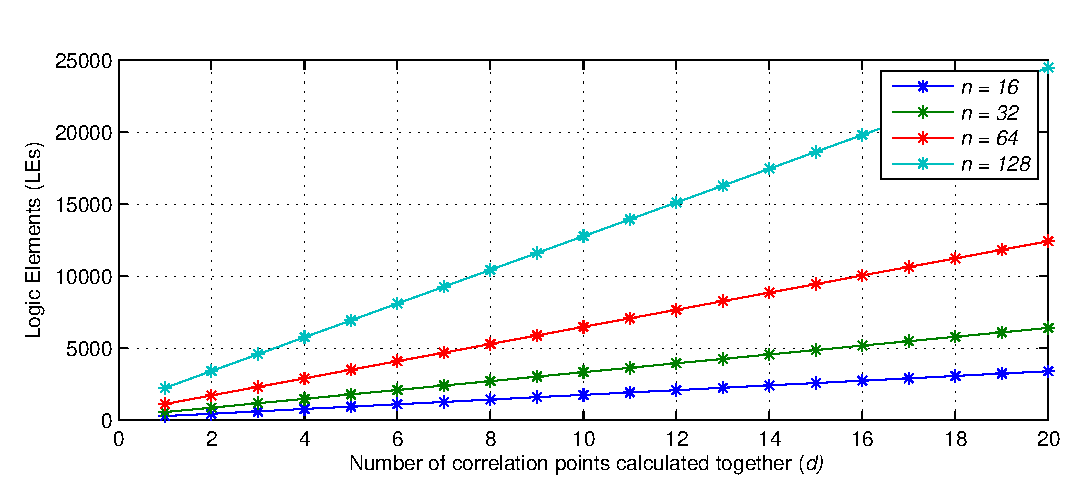
\includegraphics[width=1\linewidth]{./figures/ppt_correlator_perf_16b}
%   \caption{A subfigure}
%   \label{fig:sub1}
% \end{subfigure}%
% \begin{subfigure}{.5\textwidth}
%   \centering
%   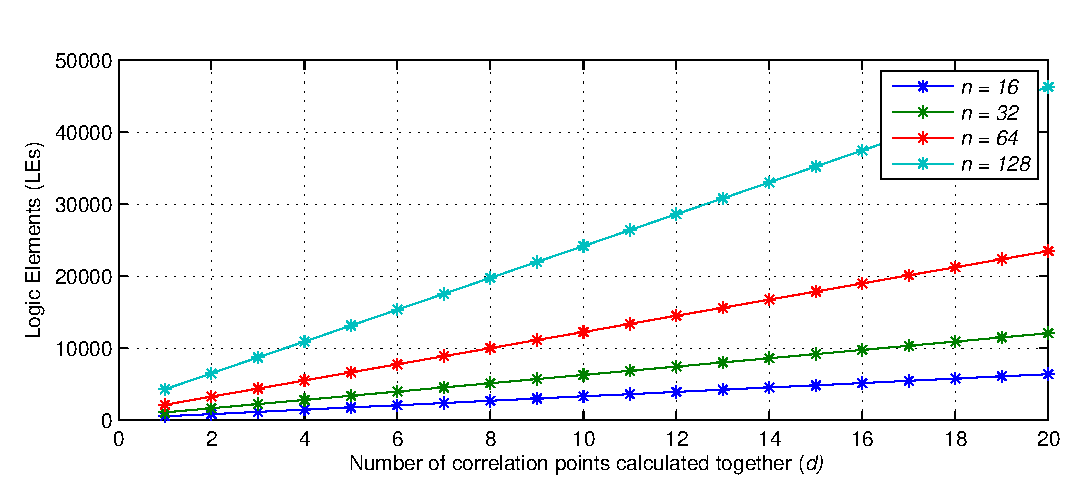
\includegraphics[width=1\linewidth]{./figures/ppt_correlator_perf_32b}
%   \caption{A subfigure}
%   \label{fig:sub2}
% \end{subfigure}
% \caption{A figure with two subfigures}
% \label{fig:test}
% \end{figure}

 \begin{figure}[!hbt]
  \centering
    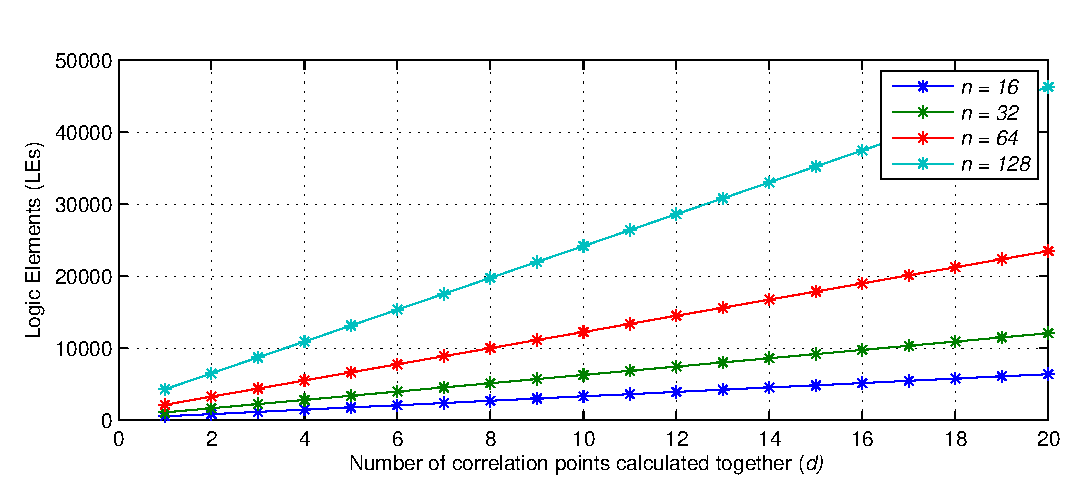
\includegraphics[width=0.9\textwidth]
      {./figures/ppt_correlator_perf_32b}
%     \rule{35em}{0.5pt}
  \caption{Altera's PPT Correlator LEs}
  \label{fig:ppt_correlator_les}
\end{figure}
 
%  \begin{figure}[!hbt]
%   \centering
%     \includegraphics[width=0.8\textwidth]
%       {./figures/ppt_correlator_altera}
% %     \rule{35em}{0.5pt}
%   \caption{Altera's PPT Correlator Architecture}
%   \label{fig:ppt_correlator}
% \end{figure}
 

% \begin{table}[htb]\small
% \centering
% \caption{LEs consumed by the complex multiplier and PPT Correlator}
% \label{table:les_ppt_complex_mult}   
% \begin{tabular}{lllllll}
% \hline
% Entity		         & \thead{Samples processes \\ together ($n$)}	& \thead{Correlation points\\ calculated together ($d$) }  		& 	\thead{ Lenght  \\ (L)}			& \thead{Bitwidth \\ (b)} &  \thead{Logic Elements \\ (LEs)}	\\ \hline
% \textbf{ICFO}              			& \textbf{973.8}			& \textbf{1769}			& \textbf{772}		& \textbf{16128}   	\\ 
% Peak Search			&\hspace{0.3cm}473   	&\hspace{0.3cm}909  		&\hspace{0.3cm}665		& 		-			    \\
% Multiplier/Conjugate      &\hspace{0.3cm}465 		&\hspace{0.3cm}798  		&\hspace{0.3cm}86 		& \hspace{0.3cm}7680  	\\

% FIFO Memories	     	 	&\hspace{0.3cm}35.8 	&\hspace{0.3cm}62			&\hspace{0.3cm}21		& \hspace{0.3cm}8448	\\
% \hline

% \end{tabular}
% \vspace{-0.3cm}
% \end{table}

% The result of equation~\ref{eq:LEs} is of $4574.1$, but since our data is complex, i.e in phase
%  and quadrature component, the result is multiplied by two, therefore the total number of logic 
% elements needed by the correlator is of $9148.2$. Comparing this result with the result 
% obtained by the logic synthesis in FPGA (table~\ref{table:results_fpga_cfo_by_entity}) we see that the total
% number of ALMs, of the complex multiplier (the only block that different in the two designs) is
% of 10. Each ALM is approximately $2.65$ logic elements for a Cyclone V device, thus the total 
% number of logic elements in the complex multiplier is of $26.5$. That is a difference of $9121.5$
% logic elements, so we can conclude that this architecture saves alot of resources.   
 
 \begin{figure}[!hbt]
  \centering
    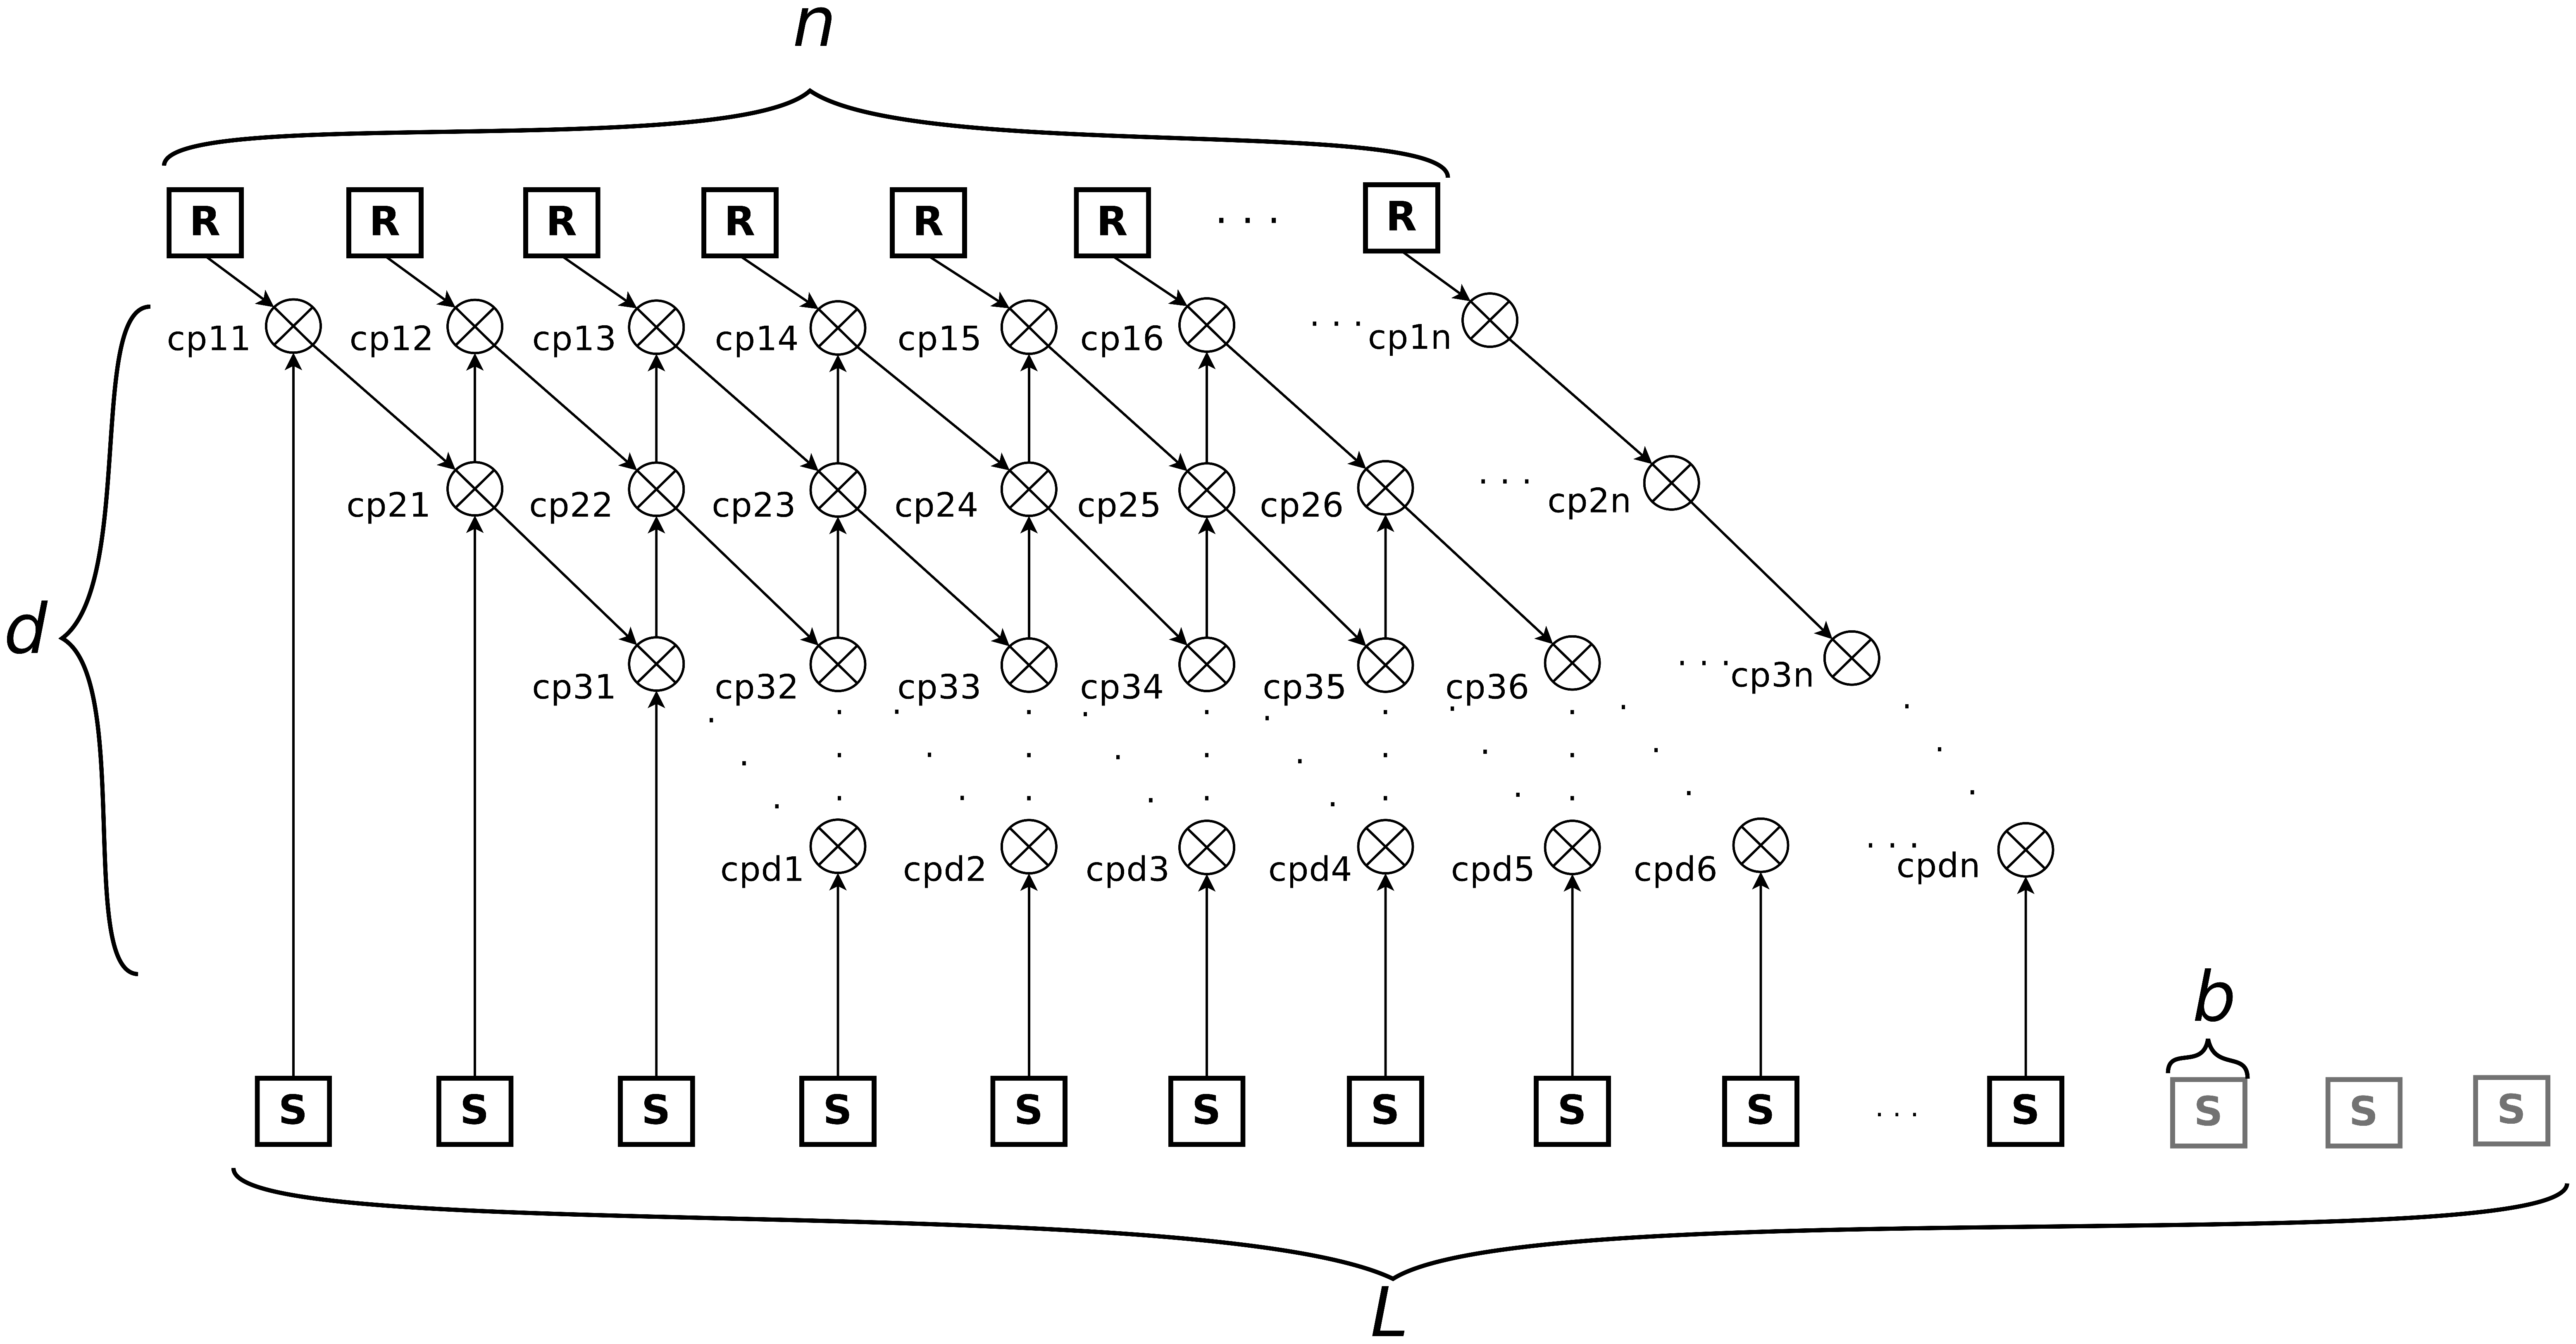
\includegraphics[width=1\textwidth]
      {./figures/ppt_correlator_altera.eps}
%     \rule{35em}{0.5pt}
  \caption{Altera's PPT Correlator Architecture}
  \label{fig:ppt_correlator}
\end{figure}
 
 
 
 
 
\begin{figure}[!hbt]
  \centering
    \includegraphics[width=0.8\textwidth]
      {./figures/int_cfo_arch_2}
%     \rule{35em}{0.5pt}
  \caption{Integer carrier frequency offset estimator/corrector with correlator}
  \label{fig:arq_cfo_2}
\end{figure}



\section{ICFO and STO }

Since the first step in the OFDM synchronization process is the timing synchronization and at this stage channel impairments, noise and CFO is still present in the signal, perfect timing estimation is always difficult to achieve. Algorithms that estimate the timing offset are not robust and residual time offset is often not entirely corrected.  


A more realistic approach to the ICFO estimation is to take into account this residual offset, in figure~\ref{fig:xcorr_sfo_exm} the results of the simulation for the FFT based correlation algorithm for a signal with STO of type II is shown. As can be seen, the correlation result does not yield a maximum value, hence not being able to find the ICFO. This is due to the shifting of the sequence in time, since the data is shifted regarding the LTF reference, the pointwise multiplication performed in time domain does not yield the same result. %Alternatives and analysis of results based on the hardware costs of this and others methods are presented briefly in the next section. 


\begin{figure}[hbt]
  \centering
    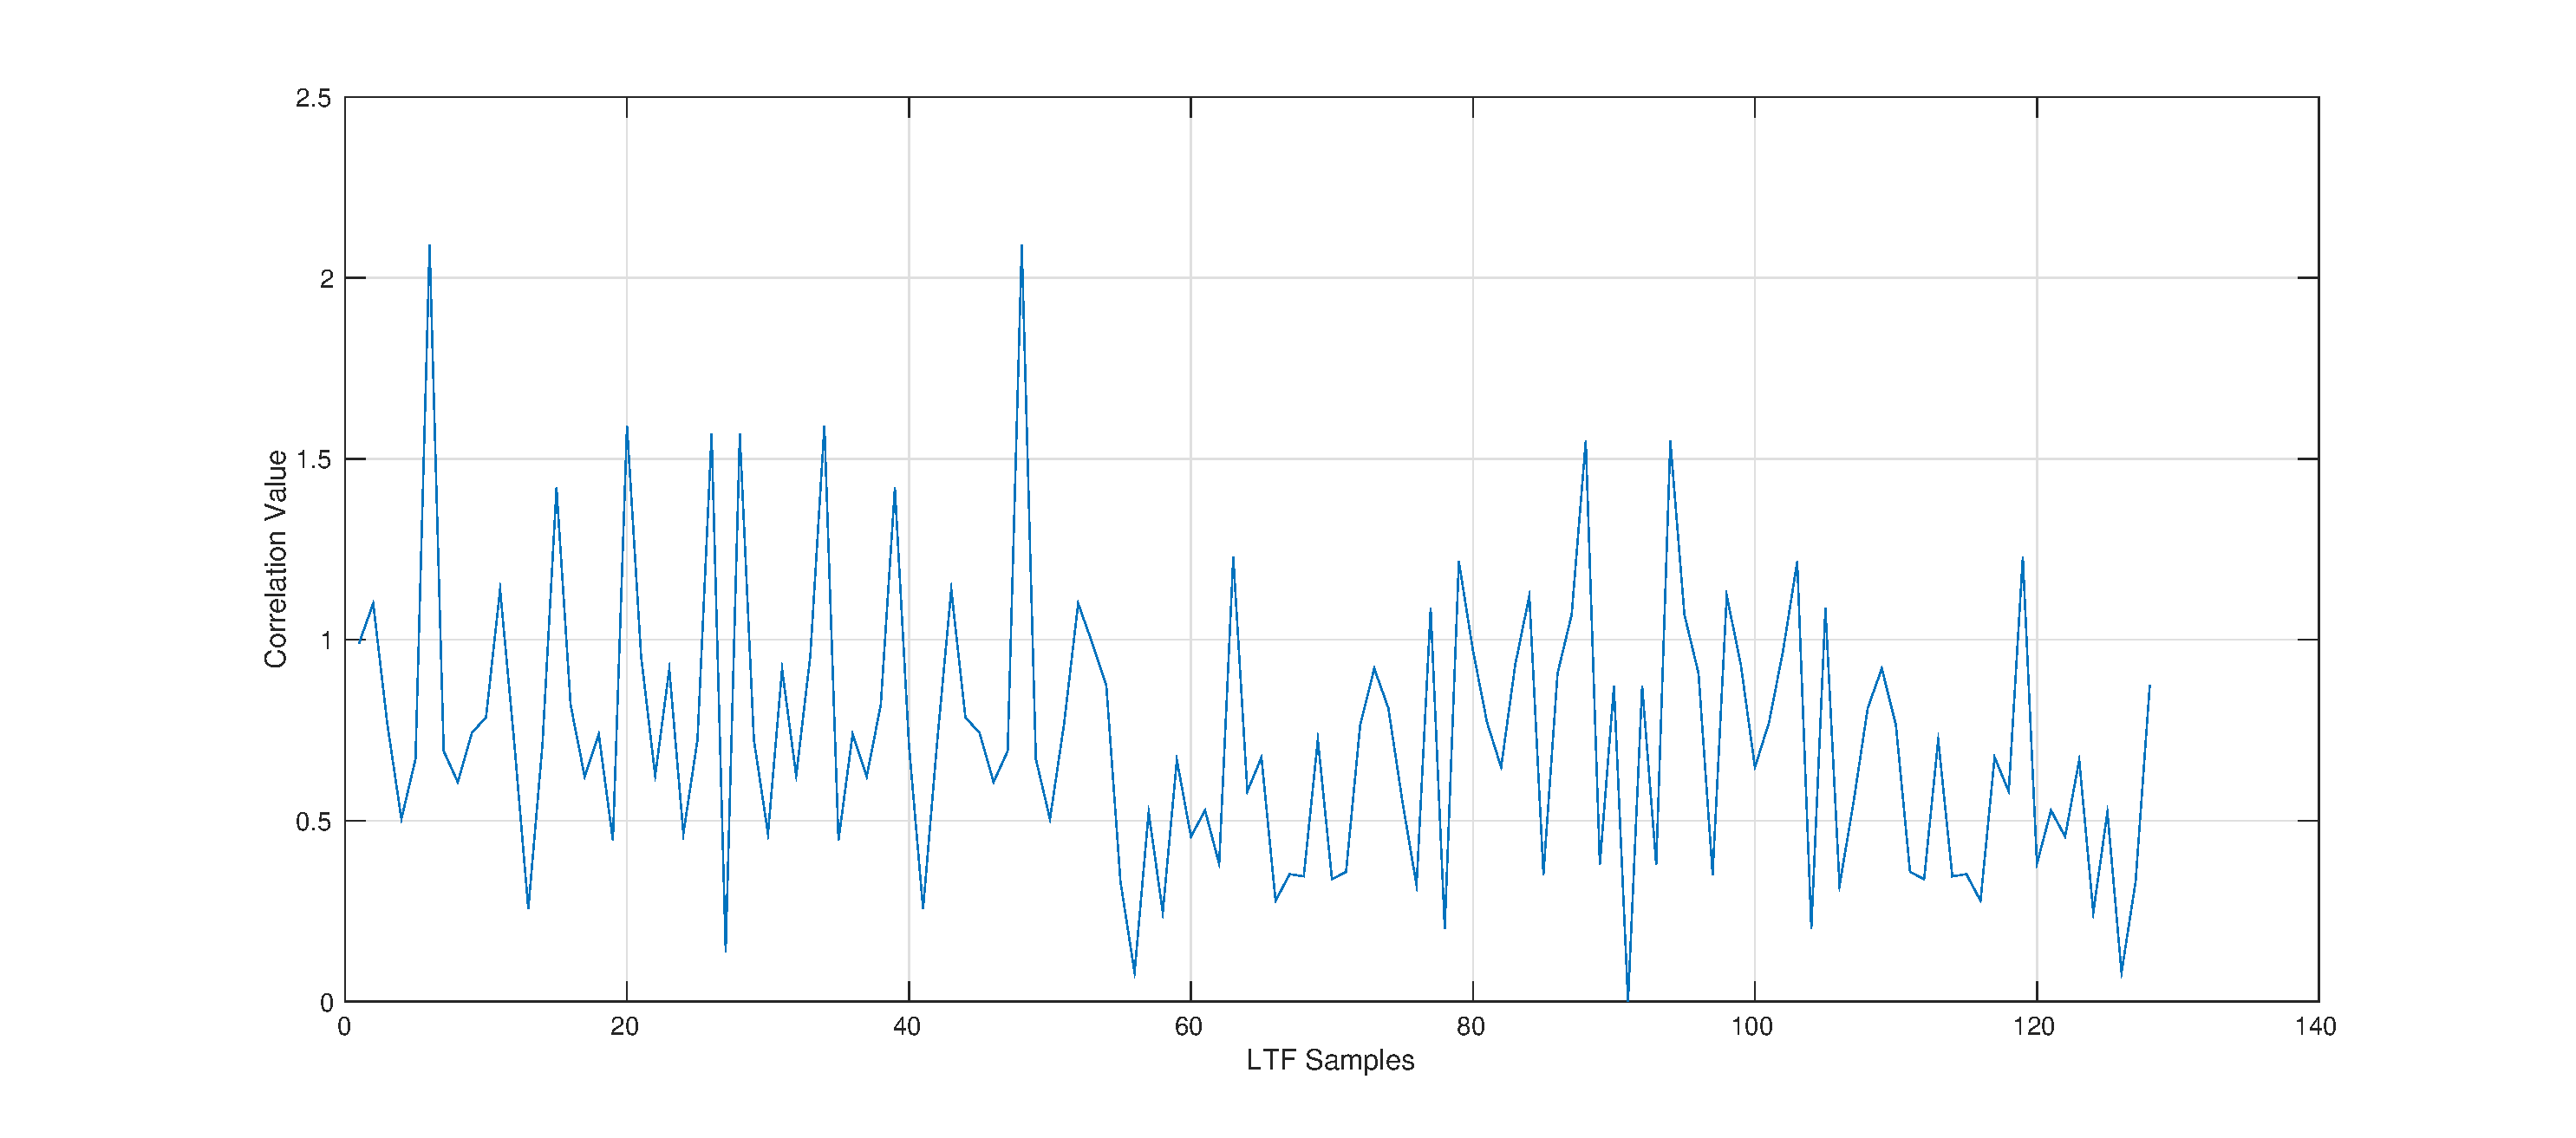
\includegraphics[width=1\textwidth]
      {./figures/correclation_result_sz128_err33_sto}
%     \rule{35em}{0.5pt}
  \caption{LTF Cross-Correlation output with SFO}
  \label{fig:xcorr_sfo_exm}
\end{figure}

\subsubsection{Canet Fine STO estimation}
An algorithm that tries to estimate this residual time offset is presented in~\cite{time_sync_canet}, Canet shows a data aided fine time synchronization method based on the cross-correlation for the IEEE802.11a/g standard, a standard that has a similar PPDU structure than that of the IEEE802.15.4g. Here, fine time synchronization is performed using a cross-correlation between the first 32 samples of the LTF sequence in time domain of the IEEE802.11.ag standard, as in eq~\ref{eq:xcorr_canet_fine_time}. 

 \begin{equation} 
%    y_n=\textbf{\textit{x}}^\intercal_n\cdot \textbf{\textit{w}}_n
C_n = g_{32}^{H}r_n
    \label{eq:xcorr_canet_fine_time}
\end{equation}


\begin{equation}
     r_n=\begin{bmatrix}
         r_{n} & r_{n+1}  & \cdots &  r_{n+31}
        \end{bmatrix}^{T}
\end{equation}

\begin{equation}
     g_{32}=\begin{bmatrix}
         LS_{0} & LS_{1} &  \cdots &  LS_{31}
        \end{bmatrix}^{T}
\end{equation}

Where $r_n$ is the received signal and $g_{32}$ are the first 32 samples of the LTF sequence, the result of the correlation for a fine STO of 10 samples, a signal without ICFO and 20db of noise is shown in figure~\ref{fig:xcorr_sfo_exm_canet}, clearly the correlation output shows a peak value at sample \emph{correlation size - STO}, sample 22 in this case. Results for a noisy channel and type II STO (refer to~\ref{sec:symbol_time_offset}) for a 128 size symbol and CP $1/4$ of symbol size with no ICFO is shown in figure. Two scenarios where tested, in the first the range of the STO is constrained to the CP size (32 samples), that is, the STO varies between 1 samples and 32 samples, on the second the size of the STO is constrained to only 16 samples. It is worth noticing that this algorithms does not works well for STOs greater than half the CP size, as can be seen from the results, a perfect estimation is only achievable when the STO is between 1 and 16 samples. Although good performance under a noisy environment is achieved with this algorithm, it does not work with ICFO as mentioned in~\ref{fig:xcorr_sfo_exm_canet}, so it must be compensated before the fine STO estimation. 




\begin{figure}[hbt]
  \centering
    \includegraphics[width=1\textwidth]
      {./figures/fine_sto_example_80211}
%     \rule{35em}{0.5pt}
  \caption{Example of the computation of fine STO by Canet Method}
  \label{fig:xcorr_sfo_exm_canet}
\end{figure}


\begin{figure}[hbt]
  \centering
    \includegraphics[width=1\textwidth]
      {./figures/fine_sto_canet_32.eps}
%     \rule{35em}{0.5pt}
  \caption{Probability of Success in Canet STO Estimation Algorithm (STO of 32 samples)}
  \label{fig:xcorr_sfo_exm_canet}
\end{figure}


\begin{figure}[hbt]
  \centering
    \includegraphics[width=1\textwidth]
      {./figures/fine_sto_canet_16.eps}
%     \rule{35em}{0.5pt}
  \caption{Probability of Success in Canet STO Estimation Algorithm (STO of 16 samples)}
  \label{fig:xcorr_sfo_exm_canet}
\end{figure}


% \begin{figure}
% \centering
% \begin{subfigure}{.5\textwidth}
%   \centering
%   \includegraphics[width=1\linewidth]{./figures/fine_sto_canet_16}
%   \caption{An STO of 16 samples}
%   \label{fig:sub1}
% \end{subfigure}%
% \begin{subfigure}{.5\textwidth}
%   \centering
%   \includegraphics[width=1\linewidth]{./figures/fine_sto_canet_32}
%   \caption{An STO of 32 samples}
%   \label{fig:sub2}
% \end{subfigure}
% \caption{Probability of success for the Canet STO estimation algorithm}
% \label{fig:test}
% \end{figure}


%results in~\cite{time_sync_canet}, show good performance is achieved with this method, it does not work with CFO. The ambiguous problem is present in the time domain, frequency errors hinders the computation of the STO in time domain, and STO hinders the computation of the CFO in frequency domain. 

%Another approach would be to try to estimate a fine time offset, a more precise time estimation to have certainty that the point chosen is the exactly the symbol start. One approach could be to find the residual time offset in frequency domain aided by the training sequences as proposed in~\cite{doc_thesys_sync}. 

\subsubsection{Non Data Aided STO Estimation}
Repetitive structures in the received signals can be used to decide the symbol start, as is the case of the CP, that repeats itself since a copy of the OFDM symbol is pre-pended to itself to avoid ISI. Algorithms that behave this way are called Non Data Aided or blind synchronization algorithms since no known sequence is used to estimate the symbol start. Although this kind of algorithms are suitable for continuous transmissions and the IEEE802.15.4g standard defines a packet by packet oriented protocol, its analysis determines the difficulty of the estimation of the fine symbol start problem.   


In Non-data aided or blind STO CP based algorithm usually two sliding windows spaced by the symbol length are correlated in time domain. In~\cite{cho2010mimo} an STO estimation technique using the symbol CP is presented, it estimates the STO by taking the difference between the two halves of the size of the CP separated by the symbol size, equation~\ref{eq:diff_cp} shows the operation. In eq.\ref{eq:diff_cp}, $y_{l}$ is the received noisy signal, $N_{cp}$ is the CP size, $N$ the symbol size and $\hat{\sigma}$ is the estimated time offset from a set of $\Sigma$ possible values. Therefore, when the difference between the two halves is minimum the similarity between them is maximum yielding the starting point. This algorithm shows immunity to CFO. Figure \ref{fig:sto_esti_cp_sqrt_diff_example} shows an example of the square difference algorithm for a time offset of 10 samples. Here, symbol size is of 128 samples and CP size 32 samples. 

 \begin{equation} 
%    y_n=\textbf{\textit{x}}^\intercal_n\cdot \textbf{\textit{w}}_n
\hat{\sigma} = \arg\min\limits_{\sigma \epsilon \Sigma} \{ \sum\limits_{n=0}^{N_{cp}-1} (| y_l[n+\sigma] |  - |y_{l}^{*}[n+\sigma+N]|)^2  \}
    \label{eq:diff_cp} 
\end{equation}

\begin{figure}[hbt]
  \centering
    \includegraphics[width=0.9\textwidth]
      {./figures/time_estimation_example_cps_diff}
%     \rule{35em}{0.5pt}
  \caption{Example of the results of the square difference algorithm}
  \label{fig:sto_esti_cp_sqrt_diff_example}
\end{figure}

Another blind algorithm that shows immunity to CFO is presented in \cite{doc_thesys_sync}, it estimates the starting point by using the auto-correlation function. The operation is shown in eq.~\ref{eq:acf_cp}. Here, when the correlation is maximum so is the similarity between the halves. Figure \ref{fig:sto_esti_cp_sqrt_acf_example} show the results of the ACF algorithms for a time offset of 10 samples. A symbol size of 128 and 32 samples of CP are used.   

\begin{equation} 
%    y_n=\textbf{\textit{x}}^\intercal_n\cdot \textbf{\textit{w}}_n
\hat{\sigma} = \arg\max\limits_{\sigma \epsilon \Sigma}  \{ |\sum\limits_{n=0}^{N_{cp}-1} ( y_l[n+\sigma]y_{l}^{*}[n+\sigma+N]) | \} 
    \label{eq:acf_cp} 
\end{equation}

\begin{figure}[hbt]
  \centering
    \includegraphics[width=0.9\textwidth]
      {./figures/time_estimation_example_cps_acf}
%     \rule{35em}{0.5pt}
  \caption{Example of the results of the auto correlation function algorithm}
  \label{fig:sto_esti_cp_sqrt_acf_example}
\end{figure}


Figure~\ref{fig:sto_esti_cp_prob_diff_acf}, shows the probability of success for the CP based methods of equations ~\ref{eq:diff_cp} and~\ref{eq:acf_cp} for a noisy channel in presence of ICFO for all OFDM Options. In this scenario a symbol taken after the SHR was used, that is all the estimations where performed adding noise to the an random generated symbol, then equation ~\ref{eq:diff_cp} and~\ref{eq:acf_cp} where used to estimate the STO. The correlated sequences sizes is of 1/4 symbol size, the size of the CP. It can be seen from figure~\ref{fig:sto_esti_cp_prob_diff_acf} that the method based on the square difference shows better performance than that of the ACF method, in fact the ACF fails at achieving an optimal estimation even for small noise values. As can be seen from fig. \ref{fig:sto_esti_cp_sqrt_diff_example} and fig.~\ref{fig:sto_esti_cp_sqrt_acf_example} a plateau is found at the minimum value of the curve for the square difference algorithm, which means that the differences between estimated values is small between adjacent $\sigma$ values, thus, the minimum value is affected greatly by noise, similar behavior can be seen for the ACF algorithm, adjacent values in magnitude of the autocorrelation show smalls differences, thus being . %Improvement in this method can be accomplished by giving a gain in the samples before performing the difference as shown in eq.\ref{eq:diff_cp_gain}, the values are then multiplied by a $H$ integer value.

% \begin{figure}[hbt]
%   \centering
%     \includegraphics[width=0.9\textwidth]
%       {./figures/prob_sucess_cp_both}
% %     \rule{35em}{0.5pt}
%   \caption{Probability of success of the CP based methods in a noisy channel}
%   \label{fig:sto_esti_cp_prob_diff_acf}
% \end{figure}

\begin{figure}[hbt]
  \centering
    \includegraphics[width=0.9\textwidth]
      {./figures/p_sucess_sto_cps}
%     \rule{35em}{0.5pt}
  \caption{Probability of success of the CP based methods in a noisy channel for all OFDM Options}
  \label{fig:sto_esti_cp_prob_diff_acf}
\end{figure}



% \begin{equation} 
% %    y_n=\textbf{\textit{x}}^\intercal_n\cdot \textbf{\textit{w}}_n
% \hat{\sigma}_{H} = \arg\min\limits_{\sigma \epsilon \Sigma} \{ \sum\limits_{n=0}^{N_{cp}-1} (H|y_l[n+\sigma] |  - H|y_{l}^{*}[n+\sigma+N]|)^2  \}
%     \label{eq:diff_cp_gain} 
% \end{equation}

%gets close to the second half, and after this occurs. So, when noise is added to the system, this minimum difference is affected by it, causing the wrong estimation value. An example of this behavior is shown in figure. On the other hand, the ACF based algorithm shows good results under a noisy environment. 

\subsubsection{Fine STO estimation in frequency domain}
A fine synchronization algorithm presented also in~\cite{cho2010mimo}, estimates the STO in frequency domain using training sequences. According to eq.~\ref{eq:symbol_rx_sto_3}, the time error introduces a phase shift that is constant, thus, if $Y[k]=Y[k-1]$, the phase difference between adjacent carriers must be equal. eq.~\ref{eq:sto_freq} shows the mathematical operation. 

\begin{equation} 
\hat{\sigma} = \frac{N}{2\pi} \arg \{  \sum\limits_{k=1}^{N-1} (Y[k]Y^{*}[k-1]  ) \}
\label{eq:sto_freq} 
\end{equation}

Since the training sequence samples are not completely equal (as required by ~\ref{eq:sto_freq}) in the LTF field  of the synchronization header for the IEEE802.15.4g standard, a slightly modification to eq.~\ref{eq:sto_freq} must be made. Taking the absolute value of every component of the complex samples yields eq.~\ref{eq:sto_freq_154g} 


\begin{equation} 
\hat{\sigma} = \frac{N}{2\pi} \arg \{  \sum\limits_{k=1}^{N-1} |\Re{(Y[k]Y^{*}[k-1])|} + |\Im{(Y[k]Y^{*}[k-1])|} \} 
\label{eq:sto_freq_154g} 
\end{equation}

The probability of correct STO estimation for the data aided phase difference in frequency domain for all OFDM Options is shown in figure~\ref{fig:sto_esti_freq_rstl}. For this algorithm the probability of success decreases with the symbol size, for smaller symbols the probability improves. The probability of success of the three STO estimation methods for a noisy channel is shown in \ref{fig:sto_esti_all_rstl} for all OFDM Options. The data aided algorithm (the phase difference in frequency domain) shows better results than the Non data Aided CP based ones, it achieves a perfect residual timing estimation for a SNR greater than 10db for the OFDM Option 4 and SNR greater than 20db for Option 1, while only the square difference algorithm achieves close to optimal optimization after only 40db.

%%%%%ONLY OPT1
% \begin{figure}[hbt]
%   \centering
%     %\includegraphics[width=1\textwidth]
%     \includegraphics[width=0.9\textwidth]
%       {./figures/p_sucess_sto_freq}
% %     \rule{35em}{0.5pt}
%   \caption{Probability of success in estimating the STO for the data aided frequency domain algorithm}
%   \label{fig:sto_esti_freq_rstl}
% \end{figure}

\begin{figure}[hbt]
  \centering
    %\includegraphics[width=1\textwidth]
    \includegraphics[width=1\textwidth]
      {./figures/p_sucess_sto_freq_ch0}
%     \rule{35em}{0.5pt}
  \caption{Probability of success in estimating the STO for the data aided frequency domain algorithm for all OFDM Options}
  \label{fig:sto_esti_freq_rstl}
\end{figure}

%%%%%ONLY OPT1
% \begin{figure}[hbt]
%   \centering
%     %\includegraphics[width=1\textwidth]
%     \includegraphics[width=0.9\textwidth]
%       {./figures/prob_sucess_cp_all}
% %     \rule{35em}{0.5pt}
%   \caption{Probability of success in estimating the STO}
%   \label{fig:sto_esti_all_rstl}
% \end{figure}


\begin{figure}[hbt]
  \centering
    %\includegraphics[width=1\textwidth]
    \includegraphics[width=1\textwidth]
      {./figures/p_sucess_sto}
%     \rule{35em}{0.5pt}
  \caption{Probability of success in estimating the STO for all OFDM Options}
  \label{fig:sto_esti_all_rstl}
\end{figure}


% \begin{figure}[hbt]
%   \centering
%     %\includegraphics[width=1\textwidth]
%     \includegraphics[width=0.8\textwidth]
%       {./figures/prob_sucess_sto_all_channel}
% %     \rule{35em}{0.5pt}
%   \caption{Probability of success in estimating the STO}
%   \label{fig:sto_methods_all}
% \end{figure}

Another factor that hinders the proper demodulation of the incoming signals that has not been taken into account is the signal degradation caused by the frequency selective channel. Simulation results for a frequency selective channel are shown in figure~\ref{fig:sto_esti_cp_diff_chn} and figure~\ref{fig:sto_esti_cp_acf_chn} for the square difference and the ACF based algorithm respectively. Both CP based algorithms show degradation in performance for a noisy and frequency selective channel, since both algorithms depend on the CP to estimate the STO.

Results for the phase difference in the frequency domain are shown in figure \ref{fig:sto_esti_ph_diff_chn}, this algorithm fails at estimating the residual STO. Not only a degradation in the estimation is shown as in the CP based algorithms, but a completely inexact estimation is shown. The probability of deviation in samples from the ideal estimated value for the frequency selective channel is shown in figure~\ref{fig:sto_esti_dev_ph_diff_chn} for a SNR of 20db. Figure~\ref{fig:sto_esti_dev_ph_diff_chn} shows that the frequency selective channel model used for this simulation introduces a phase shift in the frequency domain that is constant and that causes a different estimated value of the residual STO. 

%The estimation value given by the phase difference in frequency algorithm is then that of the phase difference caused by the STO plus a phase difference caused by the frequency selective channel. At this point it is not possible to determine the phase change introduced by the channel, thus it is not possible to estimate accurately the STO by means of the phase difference algorithm in presence of a frequency selective channel. 

% Another factor that hinders the proper demodulation of the incoming signals that has not been taken into account is the inter symbol interference caused by the frequency selective channel. Simulation results for a frequency selective channel are shown in figure~\ref{fig:sto_esti_cp_diff_chn} and figure~\ref{fig:sto_esti_cp_acf_chn} for the square difference and the ACF based algorithm respectively. Both CP based algorithms show degradation in performance for a noisy and frequency selective channel, since both algorithms depend on the CP to estimate the STO, and this is corrupted by the frequency response of the channel. Results for the phase difference in frequency domain are shown in figure x, this algorithm fails at estimating the residual STO. Not only a degradation in the estimation is shown as in the CP based algorithms, but a completely inexact estimation is shown. The probability of deviation in samples from the ideal estimated value for the current used channel is shown in figure x for a SNR of 2db. Figure shows that the frequency selective channel introduces a phase shift in frequency domain that is constant and that causes a wrong estimated value of the residual STO. At this point it is not possible to know how much the channel introduces in the phase difference estimated, therefore no compensation can be performed for this method. 


% Performance of the ICFO estimation algorithm combined with the STO estimation algorithms is shown in figure~\ref{fig:icfo_sucess_sto_correction}. The frame start is corrected according to the estimated value given by the CP and phase difference in frequency algorithms, and then the ICFO is estimated according to equation~\ref{eq:xcorr_theorem_tf}. 

\begin{figure}[hbt]
  \centering
    \includegraphics[width=0.9\textwidth]
      {./figures/p_sucess_sto_diff_cps}
%     \rule{35em}{0.5pt}
  \caption{Probability of success in estimating the STO for CP based square difference under a frequency selective Channel}
  \label{fig:sto_esti_cp_diff_chn}
\end{figure}


\begin{figure}[hbt]
  \centering
    \includegraphics[width=0.9\textwidth]
      {./figures/p_sucess_sto_acf_chn_all}
%     \rule{35em}{0.5pt}
  \caption{Probability of success in estimating the STO for CP based ACF under a frequency selective Channel}
  \label{fig:sto_esti_cp_acf_chn}
\end{figure}


%%%Only Option 1
% \begin{figure}[hbt]
%   \centering
%     \includegraphics[width=0.9\textwidth]
%       {./figures/prob_sucess_sto_ph_diff_ch}
% %     \rule{35em}{0.5pt}
%   \caption{Probability of success in estimating the STO for the phase difference in frequency domain algorithm under a frequency selective channel}
%   \label{fig:sto_esti_ph_diff_chn}
% \end{figure}

\begin{figure}[hbt]
  \centering
    \includegraphics[width=0.9\textwidth]
      {./figures/p_sucess_sto_freq_all}
%     \rule{35em}{0.5pt}
  \caption{Probability of success in estimating the STO for the phase difference in frequency domain algorithm under a frequency selective channel for all OFDM Options}
  \label{fig:sto_esti_ph_diff_chn}
\end{figure}


\begin{figure}[hbt]
  \centering
    \includegraphics[width=0.9\textwidth]
      {./figures/prob_deviation_ph_freq}
%     \rule{35em}{0.5pt}
  \caption{Probability of deviation for the phase difference in frequency domain algorithm}
  \label{fig:sto_esti_dev_ph_diff_chn}
\end{figure}

% \begin{figure}[hbt]
%   \centering
%     \includegraphics[width=0.9\textwidth]
%       {./figures/prob_sucess_icfo_w_sto_correction}
% %     \rule{35em}{0.5pt}
%   \caption{Probability of success in estimating the ICFO after computing the STO with the proposed algorithms}
%   \label{fig:icfo_sucess_sto_correction}
% \end{figure}

Results from the residual STO estimation show very poor performance for a noisy and frequency selective channel, neither the CP based approaches nor the phase difference in frequency domain approach achieves a perfect STO estimation even for low level noise, the square difference  algorithm shows the best performance of the three algorithms. The poor performance of the phase difference in frequency domain also shows that even though the estimation using this method shows a phase shift introduced by the channel in frequency domain, it not implies a displacement in the OFDM symbol samples in time domain, as it happens with the residual time offset. It is not possible to know at this point in the process the actual contribution of the channel to the phase shift estimated, hence it is impossible to compensate the error introduced by it.  


%------------------------------ICFO-----------------------------------------------------------
\subsubsection{ICFO Estimation in frequency domain with immunity to STO}

Another approach is to try to estimate the ICFO even with the residual timing error, which is the case of the work presented by BoAi in~\cite{boai_icfo}, here a data aided algorithm in frequency domain which is not affected by timing errors is presented. The operation is as described in  eq.~\ref{eq:boai_m3} 

\begin{equation} 
\hat{M} = \max\limits_{l \epsilon L}\{{\sum\limits_{k=1}^{W} | Y_{m, k}X^{*}_{m, k + l}} | \}
\label{eq:boai_m3}
\end{equation}

Here, $W$ is the number of continuous samples, $Y_{m, k}$ is the $k^{th}$ sample of the $m^{th}$ received noise corrupted OFDM symbol after the FFT, $X_{m, k}$ is the uncorrupted reference in frequency domain, $L$ is the estimation range, and $l$ the sliding window. 

\begin{figure}[hbt]
  \centering
    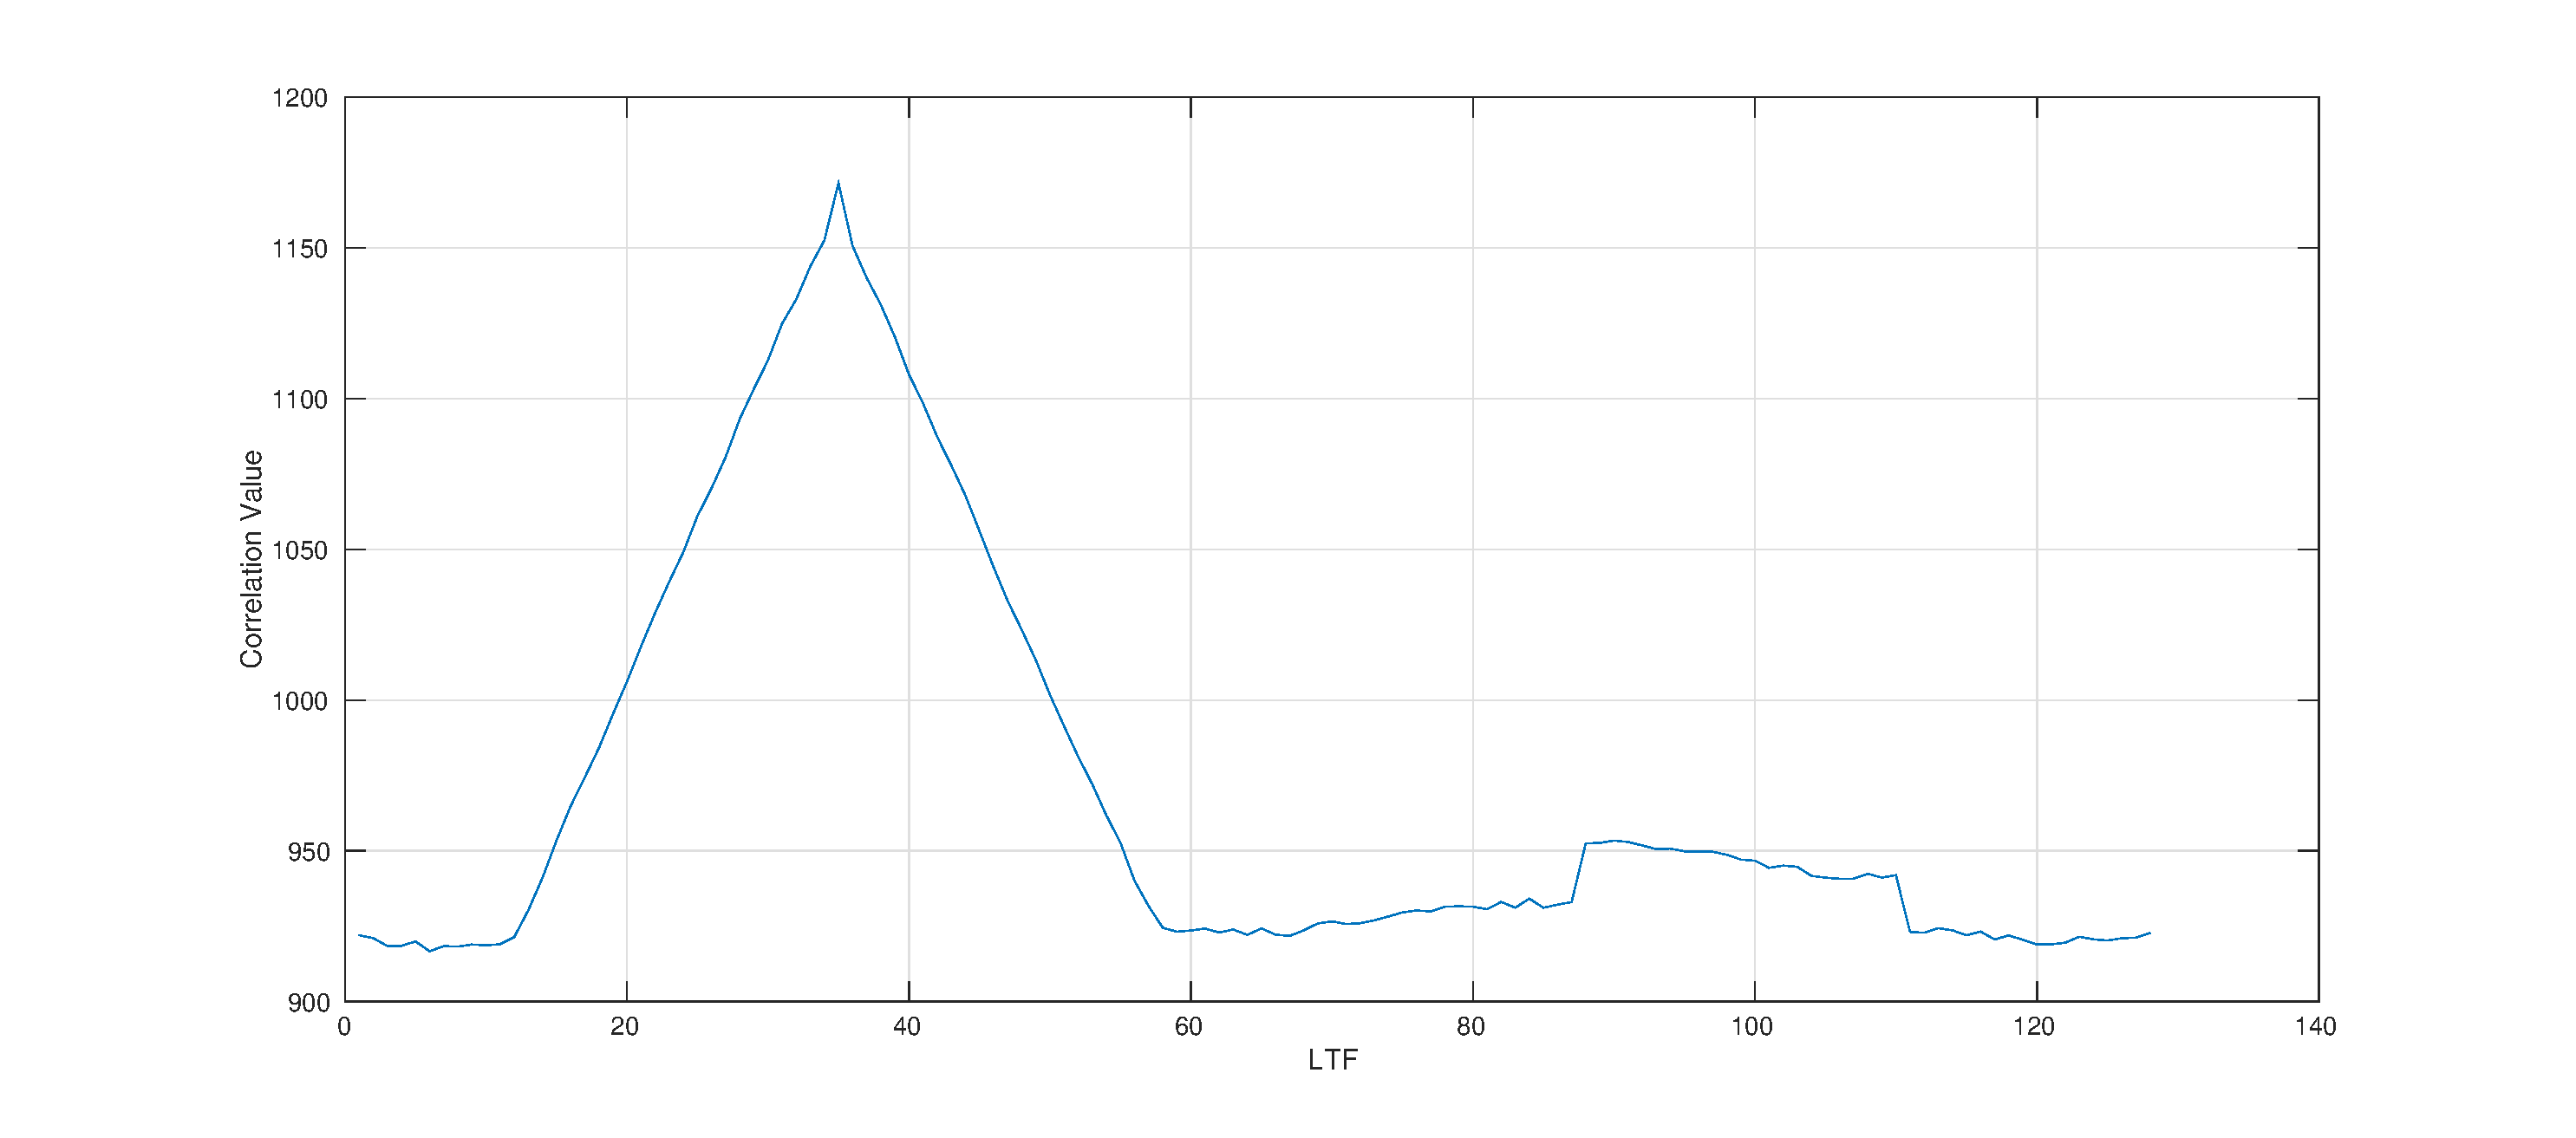
\includegraphics[width=0.9\textwidth]
      {./figures/correclation_result_sz128_err35_sto_boai}
%     \rule{35em}{0.5pt}
  \caption{Example in estimating a ICFO of 35 carriers for the BoAi Proposed Method}
  \label{fig:xcorr_boai_exm}
\end{figure}

Figure~\ref{fig:xcorr_boai_exm} shows the result of the BoAi algorithm for a residual STO no greater than the CP size, additive white gaussian noise and a ICFO of 35 subcarriers for a symbol size of 128 samples. The result of the correlations shows that a maximum peak value is found at the sample 35, the actual ICFO in the signal. 

%Performance of this algorithm is shown in figure \ref{fig:boai_probability_success}.

%As is shown in the result the estimation of the ICFO in the frequency domain taking the maximum of the correlation values is unaffected by the residual timing offset. This algorithm show good results even with STO.


\subsubsection{FFT Based ICFO Estimation with immunity to STO}
Although computing the cross correlation by means of eq.~\ref{eq:xcorr_theorem_tf} between the training sequences in presence of a small STO does not yields the actual ICFO, the correlation must yield a maximum value when the similarity between two signals is maximum. In this sense, the ICFO must yield a maximum value from within a set of maximum of correlations values. Finding the correlations of the shifted signals with STO, must yield a maximum when those signals similarities are maximized, that is when the STO is equal to zero. eq.~\ref{eq:xcorr_max} shows the mathematical operation. Here, $y(n)$ is the received long training sequence in the time domain, $x(n)$ is the reference training sequence also in time domain and $\odot$ implies pointwise multiplication between $y$ and $x$. An example of the maximum of correlations is shown in figure \ref{fig:xcorrmax_example}, here a 128 samples symbols is used, an STO of 7 samples and a ICFO of 23 subcarriers. Clearly, a peak value if found for the eighth correlation (when the STO becomes 0) in the 23rd sample of that correlation. 
%This method manages to give  



\begin{equation} 
\hat{\theta} = \max\limits_{\theta} [ \max { \mathcal{F}[y(n+\theta) \odot x^{*}(n)] }  ]
\label{eq:xcorr_max}
\end{equation}

\begin{figure}[hbt]
  \centering
    \includegraphics[width=1\textwidth]
      {./figures/max_corre_example}
%     \rule{35em}{0.5pt}
  \caption{Example of the maximum of correlations method for estimating the ICFO }
  \label{fig:xcorrmax_example}
\end{figure}


Performance of the BoAi algorithm and the maximum of correlations method for all OFDM options in presence of only white noise is presented in figure \ref{fig:boai_xcorrmax_results}. As can be seen the maximum of correlations outperforms the Boai algorithm by approximately 15 db, it reaches a perfect ICFO estimation at approximately -20db, while the BoAi algorithm at approximately -5db. Figure \ref{fig:boai_xcorrmax_results_channel_freq} shows the performance results of both algorithms without a frequency selective channel (WoC) and with a frequency selective channel (WC), here the results is almost the same as with only white noise, the frequency selective channel does not affect much the estimation for both algorithms. It is worth noticing that for the option with the least number of carriers, OFDM Option 4, the BoAi algorithms fails to estimate correctly the ICFO, this is not the case for the ICFO.  


\begin{figure}[hbt]
  \centering
    \includegraphics[width=0.9\textwidth]
      {./figures/p_sucess_icfo_all_alg_ch0}
%     \rule{35em}{0.5pt}
  \caption{Probability of success in estimating the ICFO for the BoAi and maximum of correlations Proposed Methods for all OFDM Options}
  \label{fig:boai_xcorrmax_results}
\end{figure}



\begin{figure}[hbt]
  \centering
    \includegraphics[width=0.9\textwidth]
      {./figures/p_sucess_icfo_ch_all}
%     \rule{35em}{0.5pt}
  \caption{Probability of success in estimating the ICFO for the BoAi and maximum of correlations Proposed Methods for all OFDM Options under a frequency selective channel}
  \label{fig:boai_xcorrmax_results_channel_freq}
\end{figure}

%ONLY OPTION 1
% \begin{figure}[hbt]
%   \centering
%     \includegraphics[width=0.9\textwidth]
%       {./figures/p_sucess_boai_xcorrmax_algorithms}
% %     \rule{35em}{0.5pt}
%   \caption{Probability of success in estimating the ICFO for the BoAi and maximum of correlations Proposed Methods}
%   \label{fig:boai_xcorrmax_results}
% \end{figure}



From the results obtained for the STo and ICFO estimation we can conclude that the blind techniques tested show much worse performance than that of the data aided techniques for a noisy channel, also the a robust estimation of the STO is difficult to achieve at this point in the synchronization process, channel impairments as well as frequency errors are still present in the signal making it difficult to estimate a perfect symbol time offset even for high SNR values. A small residual time offset that falls in the CP of the symbol can be corrected by the one tap equalizer~\cite{sto_equalization}, so perfect estimation is not completely needed in the OFDM synchronization process. 

% \begin{figure}[hbt]
%   \centering
%     \includegraphics[width=0.9\textwidth]
%       {./figures/prob_sucess_all_algorithms}
% %     \rule{35em}{0.5pt}
%   \caption{Probability of success in estimating the ICFO}
%   \label{fig:icfo_results_all}
% \end{figure}


% Simulations performed in the presence of additive white gaussian noise with the following parameters, FFT size $128$, sampling frequency of $fs = 1.33 Mhz$, length of CP of $16$ samples and subcarrier space $10.4 Khz$ gives the results of figure. 

% Figures show the impact of the different algorithms in the overall OFDM system performance. Here, for a SNR of x, the BER is x for the maximum of correlation algorithms, an improvement of N DBs when compared with BoAi method, and of x dbs when compared with the fine STO estimations method. Good performance is achieved with the proposed method, in the next section the hardware implementation costs of the presented methods is analyzed. 

%\section{ICFO algorithms implementation}

\section{STO and ICFO hardware implementations}

In this sections the cost of implementation of the previously presented methods for estimating the ICFO is presented. Area and throughput are the main parameters to consider for the hardware architectures presented.


\subsection{CP Based Architectures}
As it was shown in section \ref{sec:fft_cfo_architecture}, the CP of the OFDM symbol can be used to perform a not so robust fine time estimation. Two methods where presented employing similar operations to estimate the STO, one is based on the ACF while the other takes the difference between samples. The implementation of those methods are similar in logic as we will see in the following. 


Figure \ref{fig:arq_sto_acf_serial} shows the architecture for the ACF CP Based algorithm. The computation is as follows, for every clock cycle two samples from two windows separated by the symbol size are multiplied, the multiplication result of the window sample and the conjugate sample of the CP size dislocated window, is sent to an adder that sums the current multiplication results with the previous one the result is saved in a register. CP clock cycles after, the current stored value is sent to the CORDIC in circular coordinates in vectoring mode, its output is then the module of the sum, also CP clocks cycles after the first multiplication a total sum counter (Count sums in figure \ref{fig:arq_sto_acf_serial}) is incremented. The computed module is then compared with the previous greater module found, if the current value is greater its valued is saved in \emph{reg ACF} and the current count of the count sums counter counter is saved, the process is repeated shifting the input sequence until the estimated range is reached, in that moment the current stored value of the sums counter is the estimated STO. 

The architecture in figure \ref{fig:arq_sto_acf_serial} is a serial architecture, it computes one operation per clock cycle, the total delay for the maximum CP size for the OFDM option 1 and a estimation range of 10 (a maximum STO of 10 samples) is of 320 clock cycles. 

Figure \ref{fig:arq_sto_diff_serial} shows the architecture for the square difference algorithm, the functioning of this architecture is the same as the ACF, an accumulator followed by a comparator, just that in this case the module of the samples is taken at the input. Two CORDIC blocks (one for each sample, with one of them conjugated) compute the modules input, that are then subtracted and the result finally multiplied by itself, this results then goes to the same structure as in the ACF architecture to compute the STO. The time spent in the computation is the same as in the ACF architecture, CP times the estimation range, for OFDM option 1, 320 clock cycles. 

The delay in the computation time of both architectures can be reduced by parallelizing the multiplication for the ACF and subtraction for the square difference algorithm, and example is shown in figure \ref{fig:arq_sto_cp_parallel} for the ACF architecture, here, the registers are replaced by a series of $n$ registers connected that feed $n/2$ multipliers (4 in the example) and these in turn feed a tree of $n/2-1$ adders. The delay is reduced in $CP/(n/2)$. For the square difference algorithm the multipliers are replaced by subtractors and multipliers, one pair for each complex multiplier. %Table \ref{tab:requir_logic_cp} summarizes the requirements of each architecture. The numbers in parentheses are for the parallel implementation, complex components (as in registers and adders) are counted as double, that is, for the ACF implementation the number of registers at the input (the registers storing the data) must store complex data, i. e. imaginary and real part.  


% \begin{table}[]\footnotesize
% \centering
% %\begin{adjustbox}{max width=\textwidth}
% \caption{Hardware requirements for the CP based hardware implementations}
% \label{my-label}
% \begin{tabular}{ccccccccc} 
% \hline
%                                                             & Registers & \begin{tabular}[c]{@{}c@{}}Multipliers \\ (Complex)\end{tabular} & Mutipliers & Adders & Substractor & Comparators & Counters & CORDIC \\ \hline
% ACF                                                          & 8(20)     & 1(4)                                                             & -          & 2(8)   & -           & 3           & 2        & 1      \\
% \begin{tabular}[c]{@{}c@{}}Square \\ difference\end{tabular} & 5(11)     & -                                                                & 1(4)       & 1(4)   & 1(4)        & 3           & 2        & 2     \\ \hline
% \end{tabular}
%  \label{table:requir_logic_cp}
% %\end{adjustbox}
% \end{table}


 % Two version can be considered for the implementation, a semi-parallel (since a fully parallel version would consume a great amount of resources) and serial version. Figure \ref{fig:arq_sto_cp_parallel} and figure \ref{fig:arq_sto_cp_serial} show both architectures respectively. 

\begin{figure}[!hbt]
  \centering
    \includegraphics[width=0.7\textwidth]
      {./figures/sto_arq_acf_serial}
%     \rule{35em}{0.5pt}
  \caption{Serial Architecture for the CP Based ACF algorithm}
  \label{fig:arq_sto_acf_serial}
\end{figure}


\begin{figure}[!hbt]
  \centering
    \includegraphics[width=0.7\textwidth]
      {./figures/sto_arq_diff_serial}
%     \rule{35em}{0.5pt}
  \caption{Serial Architecture for the CP Square Difference algorithm }
  \label{fig:arq_sto_diff_serial}
\end{figure}

\begin{figure}[!hbt]
  \centering
    \includegraphics[width=0.7\textwidth]
      {./figures/semi_parallel}
%     \rule{35em}{0.5pt}
  \caption{Parallel multipliers in STO ACF architecture}
  \label{fig:arq_sto_cp_parallel}
\end{figure}

% The computation is as follows, from figure \ref{fig:arq_sto_cp_serial}, a multiplication of two samples is performed, then the multiplication result enters an adder tree that outputs the partial sum result. The partial sum is stored in the register \emph{reg_sum}, then the data is shifted in the samples registers and the result of \emph{Adder3} is updated with the sum of the following four values, and \emph{reg_sum} stores the sum of the current 4 values with the previous 4 values. After $CP/4$ clocks an output of the ACF is computed, this output is then sent to the comparator that check if the current computed value is greater than the previous one, if it is, the register \emph{reg_ACF} is updated and the register \emph{reg_idx} stores the index value of the current output calculated. The process stops when the range specified is reached by the counter $\sigma$.

% The serial version logic is the same, the results of the multiplication is stored in a sum register, just that in this case, instead of $CP/4$ clocks cycles, CP clocks are needed by ACF output, only one multiplier and one adder is used.


%This block makes use of the null tones inserted before and after the 
%significant data, known as active tones, appending the correct number of null tones before and after them.

\subsection{Fine STO estimation in frequency domain Architecture} 

Figure \ref{fig:arq_fine_sto_freq} shows the architecture of the fine STO estimator in frequency domain according to equation \ref{eq:sto_freq} using the LTF known sequence, its functioning is as follows, first each carrier of the OFDM symbol in the LTF is multiplied by its conjugate adjacent subcarrier, taking the difference in angle, then the absolute value of each component of the complex signal is computed and the results accumulated for $symbol_size$ cycles (the symbol size). Finally the angle of the sum is computed by means of the CORDIC and the result multiplied by $N/(2*pi)$, this output is then the STO. The delay of this architecture is of one OFDM symbol, e.g. 128 clock cycles are needed to compute the STO for option 4. 

\begin{figure}[!hbt]
  \centering
    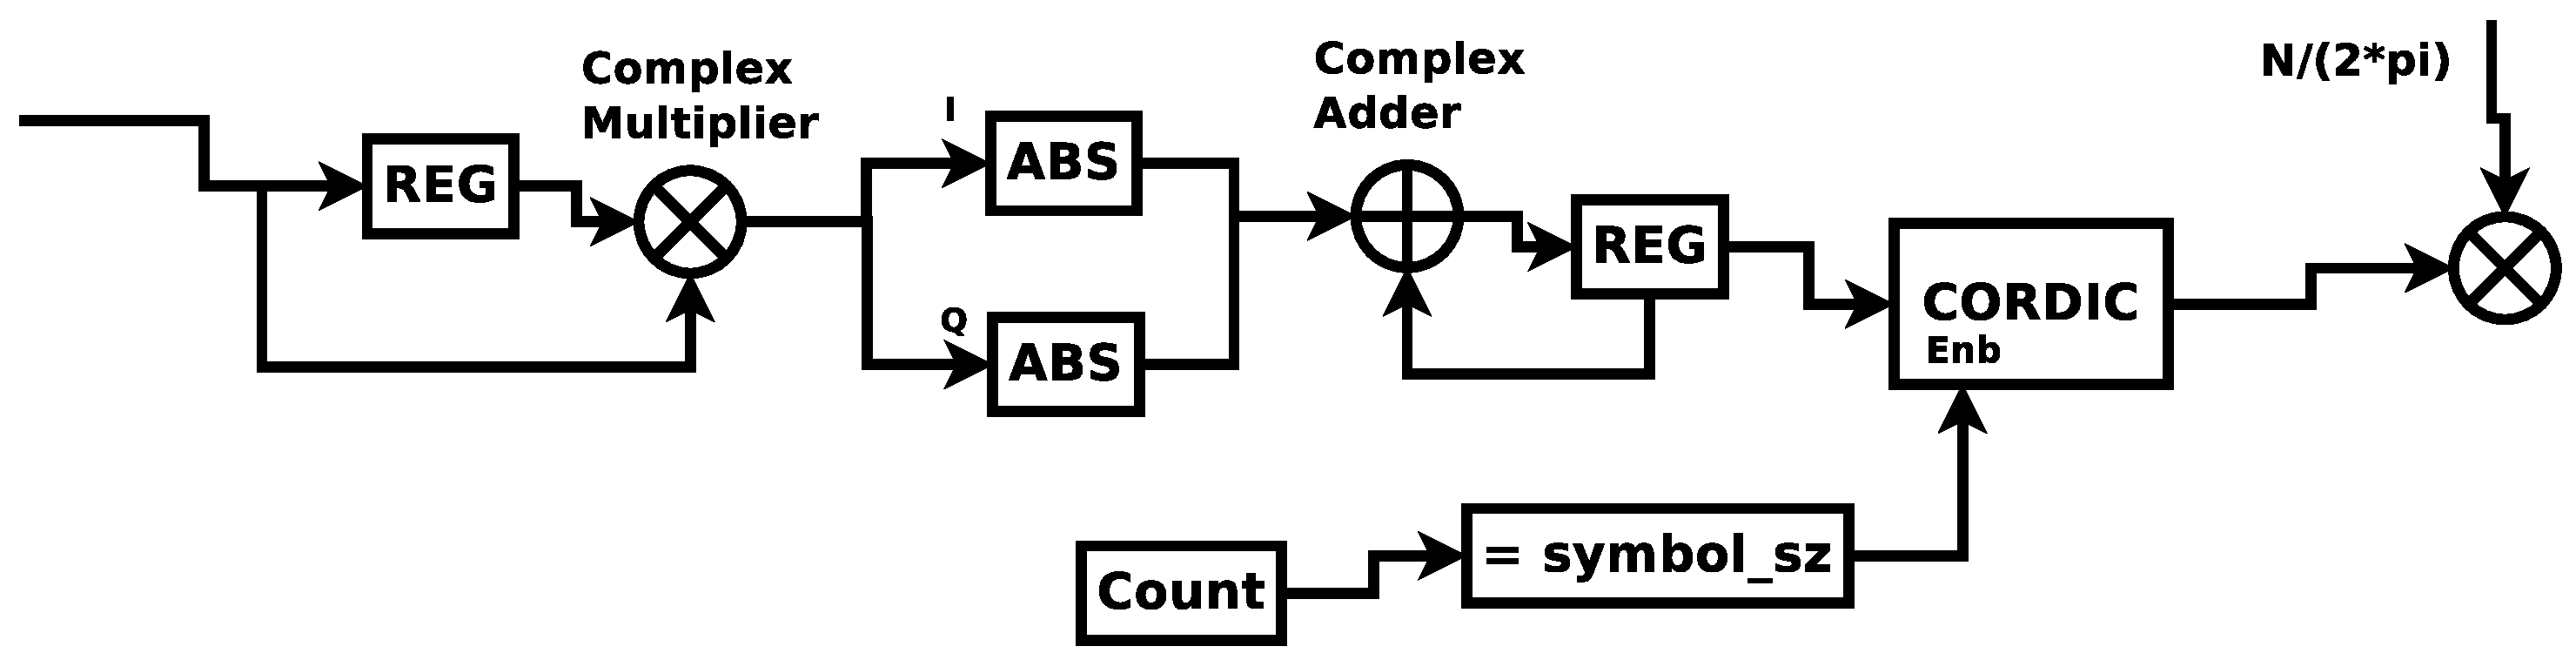
\includegraphics[width=0.9\textwidth]
      {./figures/fine_sto_freq}
%     \rule{35em}{0.5pt}
  \caption{Architecture for the Fine STO estimator in frequency domain}
  \label{fig:arq_fine_sto_freq}
\end{figure}

% \begin{table}[]\footnotesize
% \centering
% %\begin{adjustbox}{max width=\textwidth}
% \caption{Hardware requirements for the STO estimator in frequency domain}
% \label{my-label}
% \begin{tabular}{ccccccccc} 
% \hline
% %                                                             & Registers & \begin{tabular}[c]{@{}c@{}}Multipliers \\ (Complex)\end{tabular} & Mutipliers & Adders & Substractor & Comparators & Counters & CORDIC \\ \hline
% ACF                                                          & 8(20)     & 1(4)                                                             & -          & 2(8)   & -           & 3           & 2        & 1      \\
% \end{tabular}
%  \label{table:requir_logic_cp}
% %\end{adjustbox}
% \end{table}

It is worth noticing that this architecture shows poor performance under a frequency selective channel, therefore additional hardware is needed to estimate the channel and compensate its contribution to the signal phase in frequency domain in order to estimate accurately the STO. 

%As can be seen, the implementation of the square difference consumes less resources than the ACF based STO algorithm. Although it performance is lower it has some advantage over the ACF implementation, if hardware consumption is a must the square difference implementation is an option.  


\subsection{BoAi Algorithm Architecture}

 Figure \ref{fig:arq_boai} shows the BoAi implementation for the ICFO. It has some similarities with the CP based implementations, an accumulator and a register saves the current count and sends data to be compared to previous accumulated values. The computation ends when the estimation range is reached, in that moment the ICFO value is the value stores in the index registers, a registry that is updated every time a maximum value is found. 

%current value of the registers of index that is registered when an accumulator value computed is greater than the previous grater value found. 

Since the correlation of this algorithm is performed in frequency domain where the LTF is composed of +/-$1s$ and $0s$, a simpler implementation can be accomplished, the simplification comes in the multiplier at the input of the architecture, since the multiplication is performed in the frequency domain it becomes a 0 or $+1/-1$ multiplication, in hardware that can be accomplished by a series of XOR gates, one for every bit of the sample, followed by an adder. 

%The memory to store the LTF in frequency domain is also much less than that of the LTF in time domain.  

The delay of this architecture if of $128*range$ clock cycles, for example for a estimation range of $10$ subcarriers, 1280 clock cycles are required. As with the CP based architectures the process can be parallelized, XOR multipliers and CORDICs blocks in parallel (one for each sample) allows the reduction of the delay at the cost of more hardware. A parallelization of 4 samples is shown in figure \ref{fig:arq_boai_parallel}, the outputs of the CORDICs blocks are added and sent to the accumulator, the rest of the process remains the same, as with the serial case. The downside of this parallelization is the use of the CORDIC block, which uses lots of resources. The number of clock cycles is reduced to $(Symbol Size)/(parallel instances)*range$, for the example shown in figure \ref{fig:arq_boai_parallel} for a estimation range of 10 carriers,  $128/4*10 = 320$ clock cycles.  

Even though this implementation may use more sources than the STO implementations no additional hardware is required to perform the ICFO estimation, as with the STO architectures, since those architectures requires the the additional hardware of the ICFO shown in figure~\ref{fig:arq_cfo}.

%BoAi presents a simpler hardware implementation since the correlation operation is performed in frequency domain where the LTF is composed of only ones and zeros, hence simpler computations can be performed. 

\begin{figure}[!hbt]
  \centering
    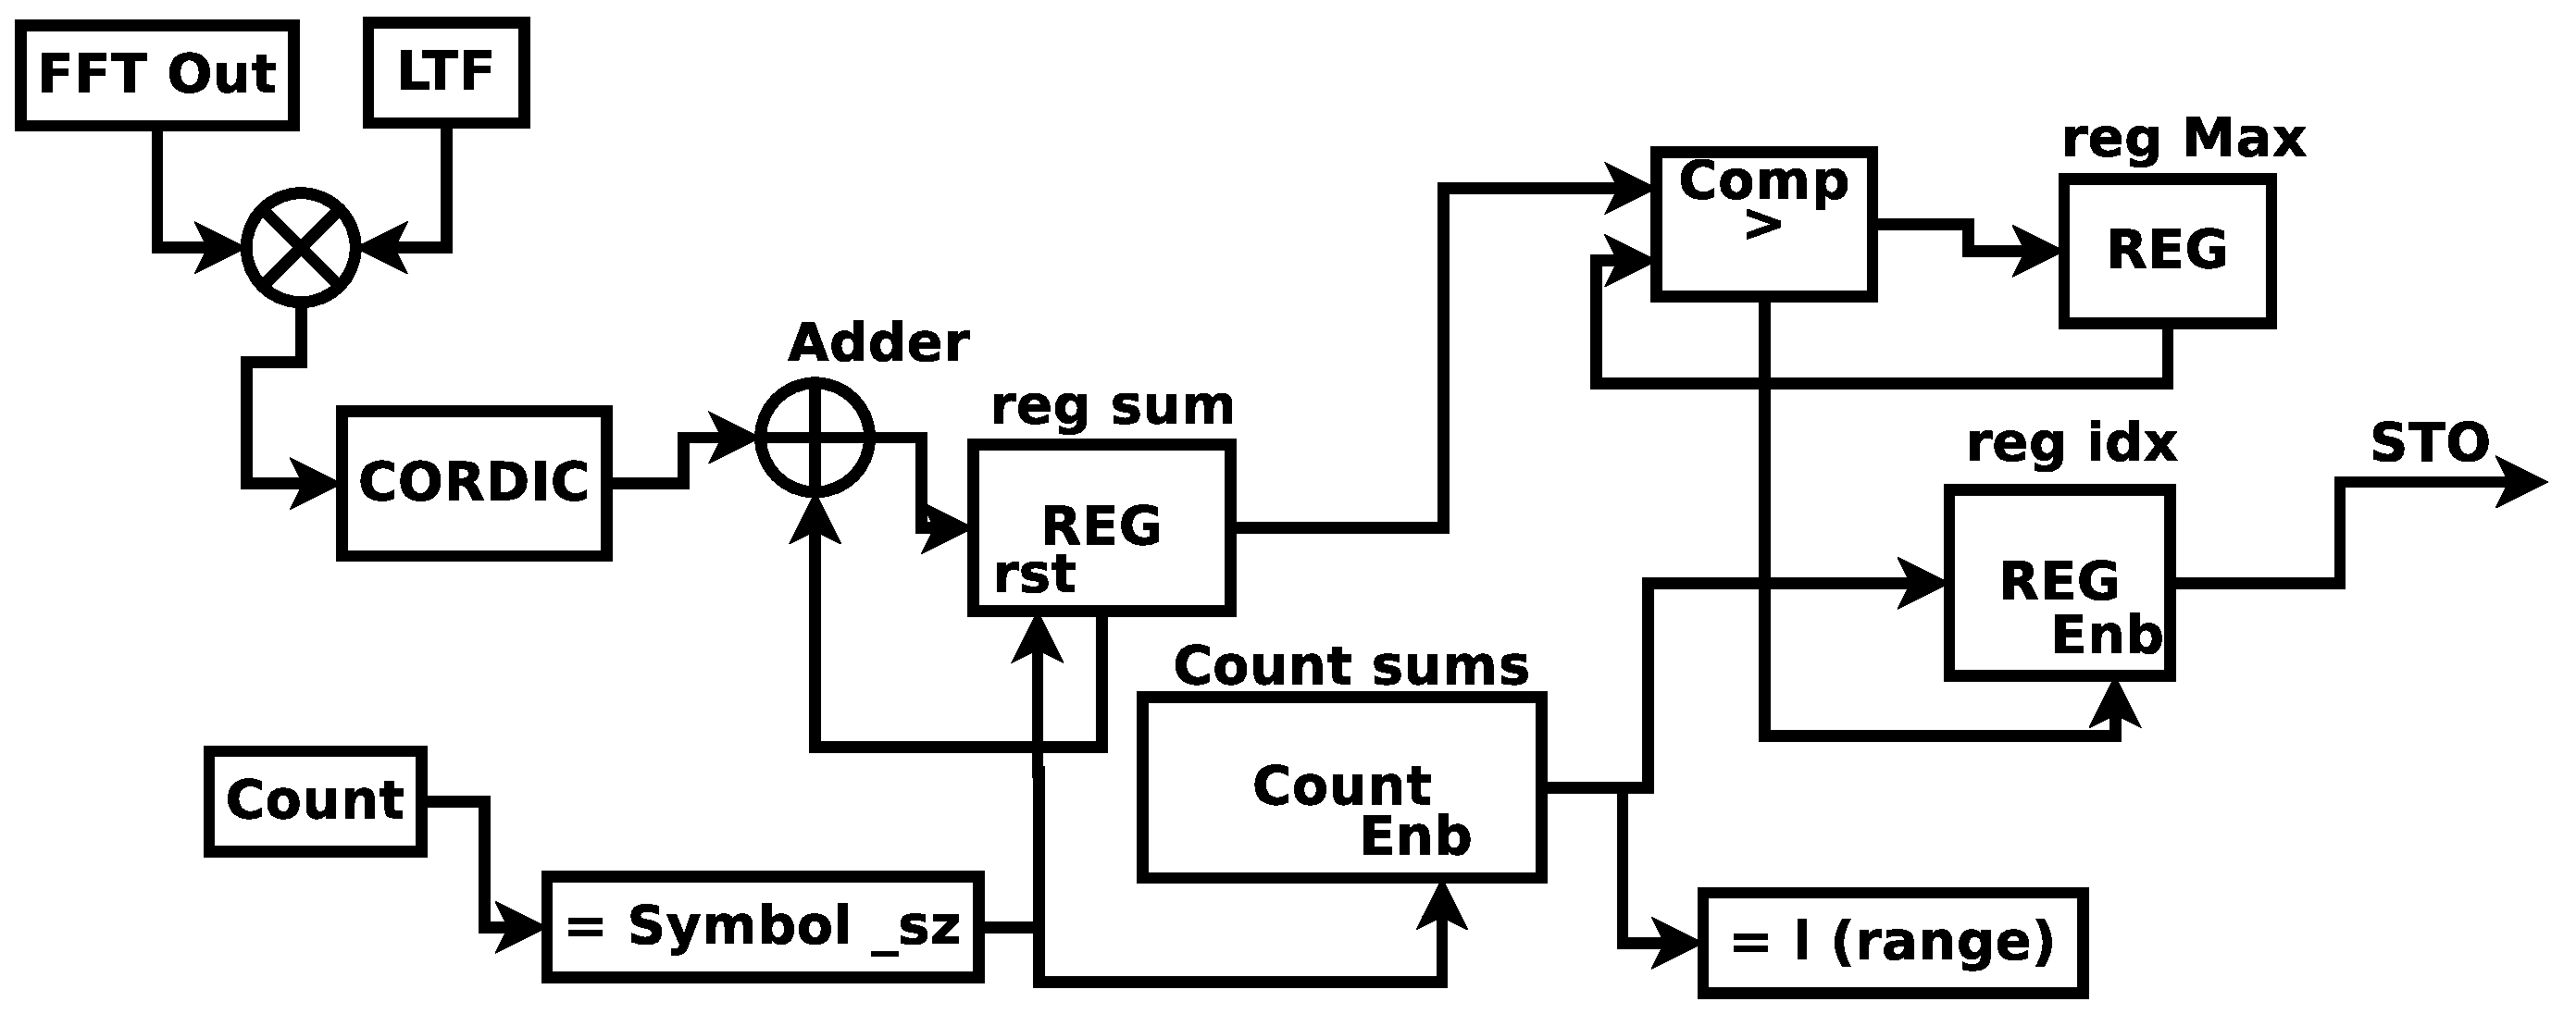
\includegraphics[width=0.7\textwidth]
      {./figures/boai_serial}
%     \rule{35em}{0.5pt}
  \caption{BoAi algorithm implementation}
  \label{fig:arq_boai}
\end{figure}


\begin{figure}[!hbt]
  \centering
    \includegraphics[width=0.7\textwidth]
      {./figures/boai_parallel}
%     \rule{35em}{0.5pt}
  \caption{BoAi algorithm implementation in parallel}
  \label{fig:arq_boai_parallel}
\end{figure}




\subsection{Maximum of correlations Algorithm}

Only a slightly modification to the implementation presented in~\ref{sec:icfo_architecture} is performed for this architecture. At the input a buffer of size $symbol size + STO range$ stores the symbol plus a small group of samples corresponding to the STO ranges to estimate, for every correlation computed the buffer shifts one sample off the buffered sequence. The symbol size sequence is then point-wise multiplied in time domain by the uncorrupted reference LTF and the result sent to the FFT block, the FFT out now goes to the peak searcher that finds a local maximum, then the buffered sequence is shifted and another correlation is computed. This local maximum is then compared with all the local maximums of all the correlations computed, the index of the maximum of local maximums (the global maximum) is the ICFO. The previously peak searcher shown~\ref{sec:icfo_architecture} must then be  changed to compute maximum of maximum values. The new peak searcher block is shown in figure \ref{fig:max_corre_peaks}.  

\begin{figure}[!hbt]
  \centering
    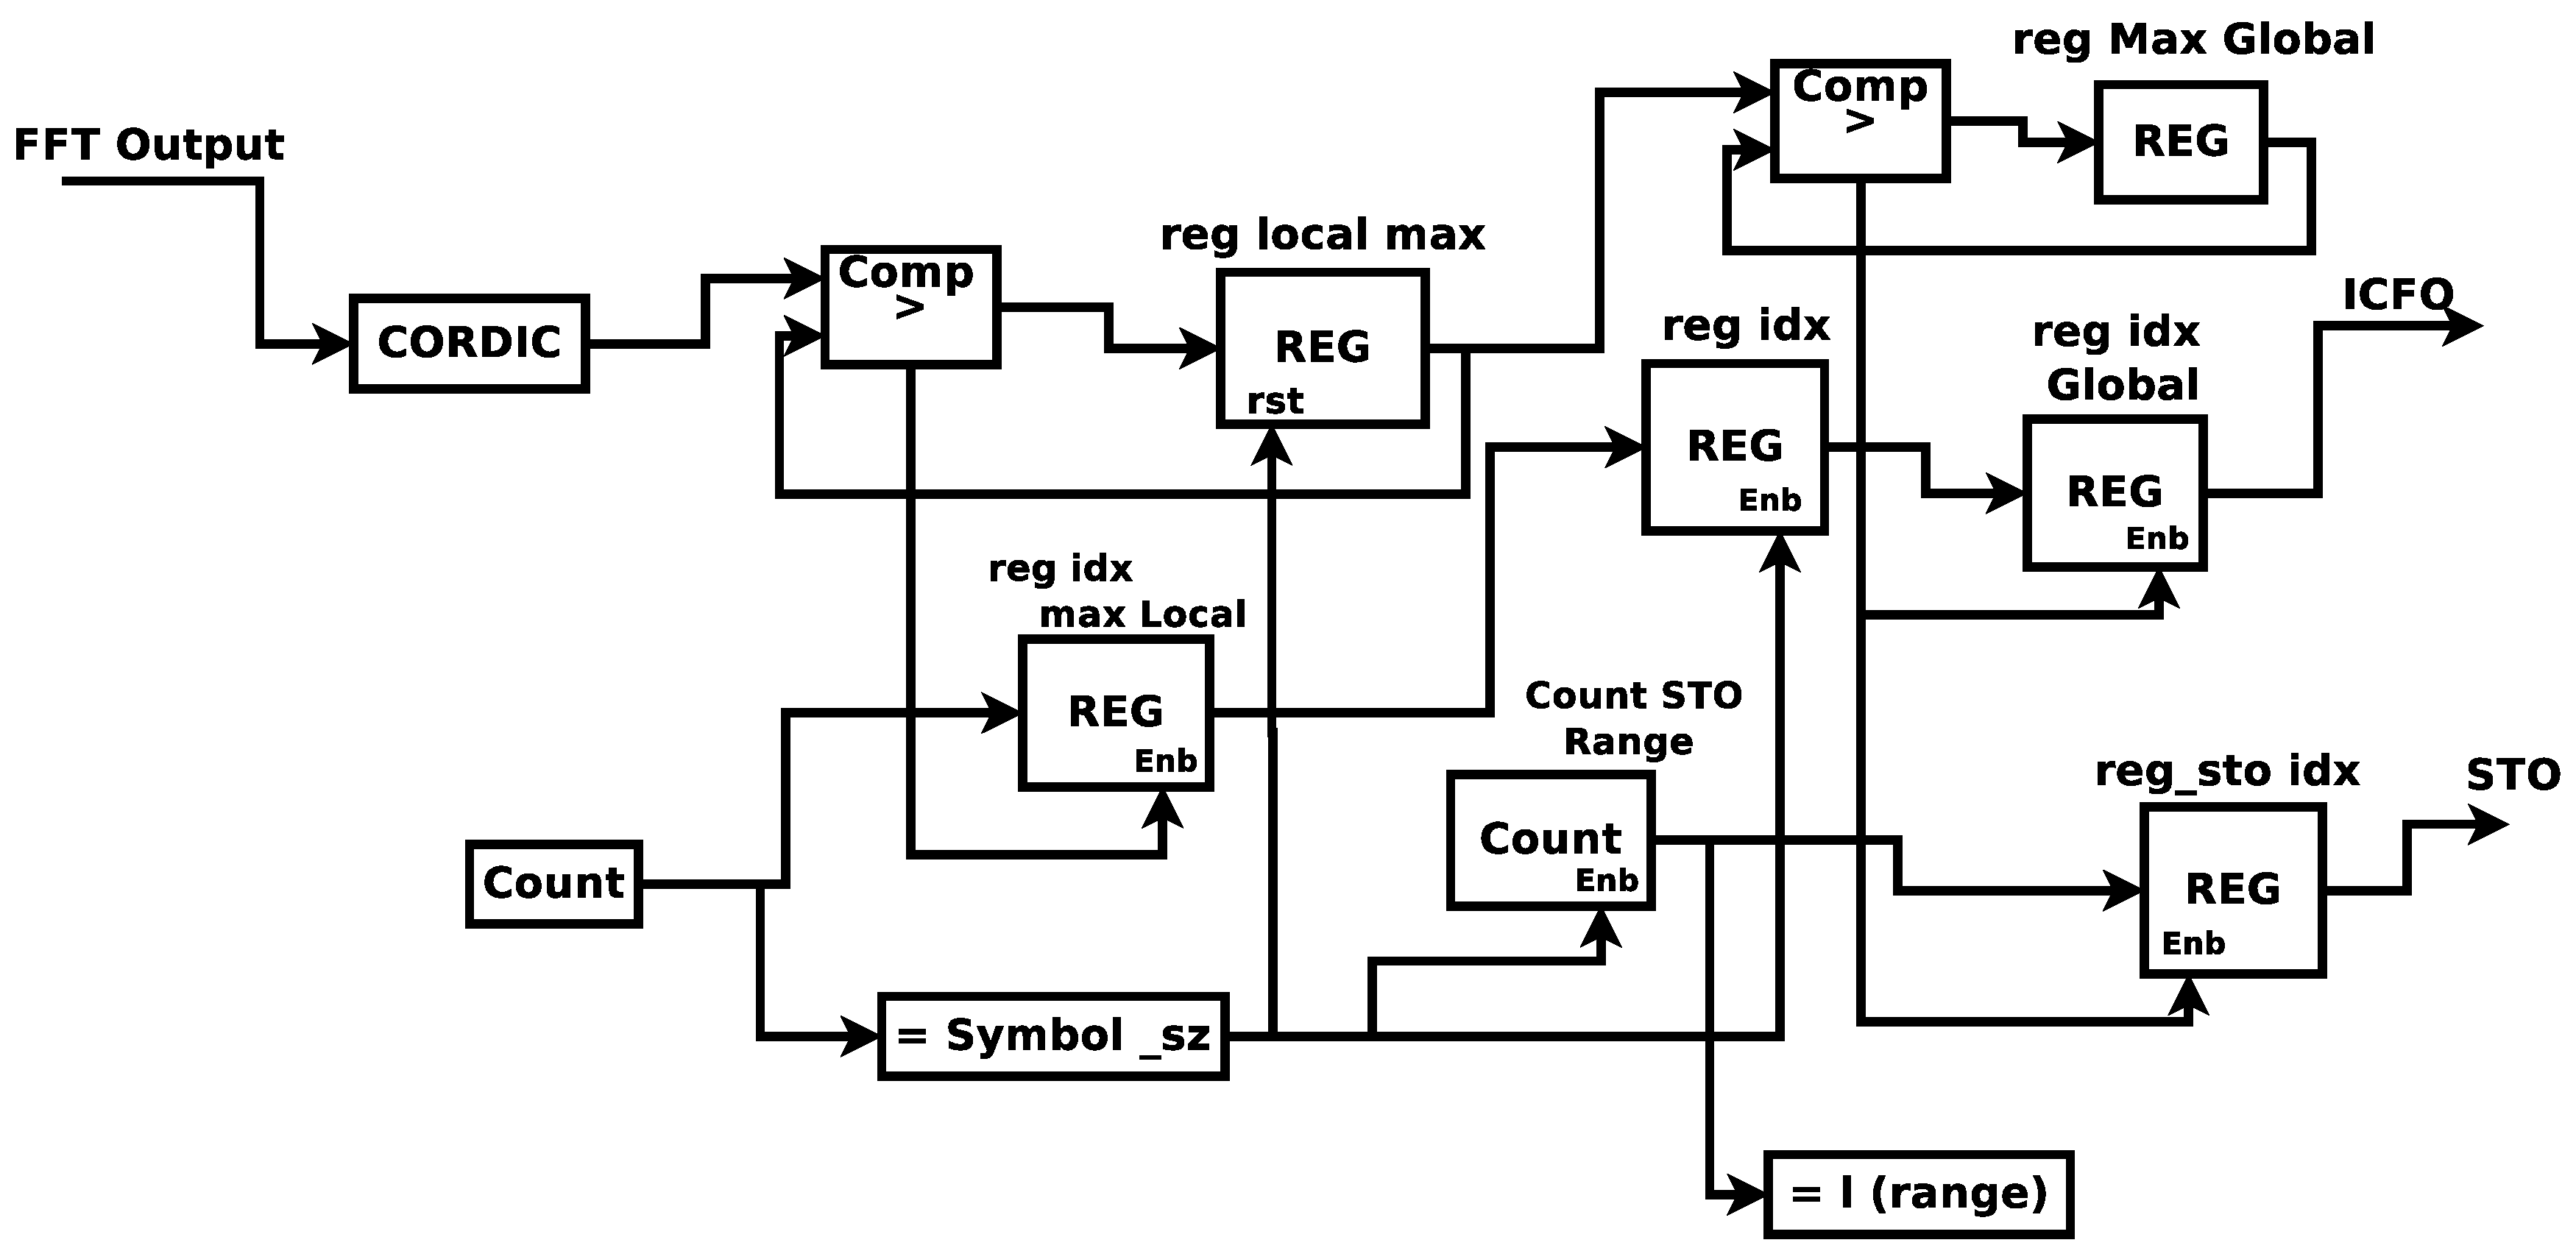
\includegraphics[width=0.9\textwidth]
      {./figures/peak_searcher_new}
%     \rule{35em}{0.5pt}
  \caption{Peak searcher for the FFT based maximum of correlations algorithm}
  \label{fig:max_corre_peaks}
\end{figure}

To find the global maximum (the maximum of the maximum of all the computed correlations) the peak searcher compares the current FFT output with the previous one, every time a maximum value is found its value is stored in the register \emph{reg local max}, in parallel the local index of where this maximum value was found is stored in the register \emph{reg idx max local}. When the samples count reaches the symbol size, the value of the maximum register along with the value of its index is passed to a global comparator that compares the current maximum local value with the previous partial global found, the index value is stores in a auxiliary register, if the current value is greater than the previous one the current value is stored and the global index register is updated with the auxiliary register value. The process ends when the STO range value is reached. 

Since the computation of the ICFO by means of this method involves the FFT computation, the delay of the computation includes the delay of the FFT, which slows down the process. For this method the delay is given by eq \ref{eq:delay_max_xcorr}.

\begin{equation} 
delay_{maxcorr} = (delay_{FFT} + Symbol_{sz})*STO_{range} 
\label{eq:delay_max_xcorr}
\end{equation}

\begin{equation} 
delay_{fft} = \frac{FFT_{sz}}{2}\log_2{FFT_{sz}}  
\label{eq:delay_max_xcorr}
\end{equation}


For a STO of 10 samples and OFMD option 1, the delay of this architecture is of $5760$ clock cycles. The delay of this architecture is the greatest of all the implementations presented. However, some modifications can be done to reduce this delay:

\begin{itemize}
\item \emph{Pipeling the FFT} : with this method the delay of the computation is reduced to $Symbol_{sz}*STO_{range}$. Although it may seem that the advantages of the FFT implementation presented previously are lost with the use of a pipeline architecture, the use of a CORDIC based butterfly that eliminates the use of ROM memories to store twiddle factors can still be used in a pipeline structure. The only disadvantage of the pipeline approach would be hardware reuse, for FFT sizes smaller than 128 much of the hardware occupied by the FFT would remain without utilization. It is worth noticing, that blocks with very large delays halt the system, requiring buffers to compensate those delays. Those buffers hardware requirements that the serial implementation introduces could be more than the size needed by the pipeline version of the FFT, thus requiring an FFT pipelined in the final design, even if there is no FFT based ICFO. A pipelined FFT would allow to implement the presented method without much delay and with advantages over other ICFO implementations, for example the ICFO range that this implementation allows is of a symbol size ($128$ for OFDM option 1), whereas the BoAi implementation requires $128*128$ to estimate the same range of ICFO. The analysis of the requirements and the benefit of the pipeline architecture in the whole MR-OFDM system is still an ongoing task.

\item \emph{Modules running at different clock frequencies} By running different modules at different clocks frequencies, a reduction in blocks delays can be achieved. If the FFT block runs at a higher frequency than that of the rest of the design, the delay of this block can be compensated, this of course has implications in power consumption. 

%the FFT delay and consequently a reduction in the ICFO delay
\end{itemize}
 
 

 %Further results and other variables in the whole design determine this tradeoff, as in the area available for the final chip and power consumption

%is a must, since the intended application is low power, and an architecture that occupies much more hardware could lead to greater power consumption. It is worth remembering that implementations of this kind are not trivial and can take months of development process, but also, the FFT is an important block in the OFDM system, time of development could lead to a much improved design.    

% \item \emph{Reduce the FFT size} : Reducing the range of the ICFO by reducing the size of the FFT computed to perform the correlation the delay can be also reduced, for example, for a 128 size FFT, only the first 32 points of the correlation are computed. This would reduce the computation time at the cost of a reduced ICFO range. 

Tables \ref{table:resources_entity_all_sto} and \ref{table:resources_entity_icfos} show a summary of the resource consumption of every architecture presented in FPGA. The table shows the architecture area consumption as well as area consumption of its most resource consumption block. These implementations are early versions of what would have been the optimal implementation for all architectures, that is no rigorous functional verification where performed on those implementation, this is due the implementations begin made only as an estimation of the hardware consumption of all the presented methods for the computation of the ICFO. It is worth noticing that the values shown in table \ref{table:resources_entity_all_sto} are for only the the STO estimation, the ICFO estimation by means of these methods (that is estimating first the STO and then the ICFO using the FFT based correlation) requires the additional hardware presented in section \ref{sec:icfo_architecture}. As can be seen from table \ref{table:resources_entity_all_sto} and table \ref{table:resources_entity_icfos} blind STO algorithms in time domain consume much more hardware than the STO method in frequency domain.  


 \begin{table}[htb]\small
\centering
\caption{Resource Utilization by Entity in the ICFO architectures}
\label{table:resources_entity_icfos}
\begin{tabular}{llccl}
\hline
Entity			                                  	&Combinational	ALUT	& Registers				\\ \hline
\tikzmark{max_corr}\textbf{Maximum of Correlations}              	& \textbf{700}(47)			& \textbf{642}(68)		 	\\ 
\hspace{0.3cm}\tikzmark{cdc4}CORDIC   	&\hspace{0.3cm}653  	&\hspace{0.3cm}574		\\
\tikzmark{boai_top}\textbf{BOAI Top}              	& \textbf{738}(52)			& \textbf{662}(56)		 	\\ 
\hspace{0.3cm}\tikzmark{cdc1}CORDIC               	&\hspace{0.3cm}653  	&\hspace{0.3cm}574	    \\
\hspace{0.3cm}\tikzmark{xor_mult}XOR Multiplier   	&\hspace{0.3cm}33  	&\hspace{0.3cm}32		\\
\hline
\tikz[remember picture] \foreach \i in {cdc1,xor_mult} \draw[overlay] (pic cs:boai_top) |- ([yshift=1.0mm]pic cs:\i);
\tikz[remember picture] \foreach \i in {cdc4} \draw[overlay] (pic cs:max_corr) |- ([yshift=1.0mm]pic cs:\i);
\end{tabular}
\vspace{-0.3cm}
\end{table}

\begin{table}[htb]\small
\centering
\caption{Resource Utilization by Entity in the STO architectures}
\label{table:resources_entity_all_sto}
\begin{tabular}{llccl}
\hline
Entity			                                  	&Combinational	ALUT	& Registers				\\ \hline
\tikzmark{cpacf}\textbf{CP ACF Top}              	& \textbf{2473}(99)			& \textbf{641}(67)		 	\\ 
\hspace{0.3cm}\tikzmark{cdc2}CORDIC               	&\hspace{0.3cm}951  	&\hspace{0.3cm}574	    \\
\hspace{0.3cm}\tikzmark{cplx_mult}Complex Multiplier   	&\hspace{0.3cm}1423  	&\hspace{0.3cm}0		\\
\tikzmark{cpdiff}\textbf{CP Diff Top}              	& \textbf{2267}(67)			& \textbf{1199}(51)		 	\\ 
\hspace{0.3cm}\tikzmark{cdc3}CORDIC               	&\hspace{0.3cm}2*951  	&\hspace{0.3cm}2*574	    \\
\hspace{0.3cm}\tikzmark{mult}Multiplier   	&\hspace{0.3cm}298  	&\hspace{0.3cm}0		\\

\hline
\tikz[remember picture] \foreach \i in {cpacf,cdc2,cplx_mult} \draw[overlay] (pic cs:cpacf) |- ([yshift=1.0mm]pic cs:\i);
\tikz[remember picture] \foreach \i in {cpdiff,cdc3,mult} \draw[overlay] (pic cs:cpdiff) |- ([yshift=1.0mm]pic cs:\i);
\end{tabular}
\vspace{-0.3cm}
\end{table}

Results presented in the previous sections shows that the choice of an optimal ICFO estimator is carried on plenty of variables to analyze, area consumption, estimation range, good performance under a noisy channel as well as immunity to multi path channel and STO are some of the variables that determine the choice of an optimal ICFO estimator. Other issues not yet analyzed could also impact the choice of a ICFO estimator, as is power consumption, that is a must for the intended application. 

The approach of estimation and correction of the STO before the ICFO computation by means of the FFT based algorithm shows poor performance for the Non data aided or blind algorithms, also, data aided algorithms show problems with channel multipath in frequency domain or more complex computations in time domain due to the complex multiplications involved in the method presented. 

The STO estimation process must deal with all the impairments in the system, since it is the first estimation performed. Although difficult, the  estimation of small STOs does not have to be perfect or exact, since the phase difference introduced by it in the frequency domain can be corrected by means of the equalization process, as long as the residual error falls inside the symbol CP.

Others methods presented that are not affected by the STO and show immunity to the multipath channel and show good performance for noisy signal are more suitable for the ICFO estimation, since less area and computation complexity is used. For the BoAi algorithm 
the multiplications performed are much less complex than those of the correlation algorithm in time domain, in performance, the maximum correlation algorithm show good results. If performance is a must it can be achieved at much less costs with the maximum correlations. Also, this method can be improved by pipelining the FFT or its delay improved by a multi-frequency design where its frequency is increased reducing the overall time spent to perform the computation. The feasibility of a pipeline implementation of the FFT must be analyzed with the whole OFDM transceiver, its consumption in area from the chip total available area as well as power consumption are two of the main parameters to consider. If good performance under noisy environment is a must, the maximum correlations algorithms is a good candidate for the ICFO estimation. Chip costs are also another variable in which the algorithms can have an impact, a better ICFO estimator can mean a cheaper oscillator crystal which means a cheaper chip.

As can be seen the choice of the optimal algorithm for the ICFO estimator an corrector depends on many variables that are unknown at this point of the project, for example chip costs and chip area. From the results obtained and the analysis performed until this point it can be concluded that the proposed method, the maximum correlations method, is an optimal choice only if performance is a must, the algorithms shows good performance for a noisy and frequency selective channel as well as immunity to residual STO. Also, the architecture can be very much improved, by different methods,  it is believed that the impact not only on the ICFO but also on the overall OFDM transceiver could compensate for the modifications in the architecture. This is a previous conclusion taken from the current available results, other variables as in other blocks performance could discard the advantages presented for the tradeoffs of the architectures i.e. if any of the other block in the receiver does not work with negative SNRs, the advantage of the current implementation with the cost of additional hardware would be lost. The overall performance would be compromised by this other block. 

%As was mentioned before, the designs can change in late stages of the ASIC design process. 

%under noisy channel well as later results of the low level synthesis could lead to more changes in those designs.  

%in hardware consumption as well as in power consumption must be determined by the lower processes of the ASIC design, where a power estimation and also on chip avalaible area   

%%%%%%%%%%%%%%%%IMPRIMIR%%%%%%%%%%%%%%%%%%%%%%%%%
% \begin{figure}[!hbt]
%   \centering
%     \includegraphics[width=0.7\textwidth]
%       {./figures/sto_arq_acf_serial}
% %     \rule{35em}{0.5pt}
%   \caption{Serial Architecture for the CP Based ACF algorithm}
%   \label{fig:arq_sto_acf_serial}
% \end{figure}


% \begin{figure}[!hbt]
%   \centering
%     \includegraphics[width=0.7\textwidth]
%       {./figures/sto_arq_diff_serial}
% %     \rule{35em}{0.5pt}
%   \caption{Serial Architecture for the CP Square Difference algorithm }
%   \label{fig:arq_sto_diff_serial}
% \end{figure}

% \begin{figure}[!hbt]
%   \centering
%     \includegraphics[width=0.7\textwidth]
%       {./figures/semi_parallel}
% %     \rule{35em}{0.5pt}
%   \caption{Parallel multipliers in STO ACF architecture}
%   \label{fig:arq_sto_cp_parallel}
% \end{figure}

 
% \begin{figure}[!hbt]
%   \centering
%     \includegraphics[width=0.7\textwidth]
%       {./figures/boai_serial}
% %     \rule{35em}{0.5pt}
%   \caption{BoAi algorithm implementation}
%   \label{fig:arq_boai}
% \end{figure}


% \begin{figure}[!hbt]
%   \centering
%     \includegraphics[width=0.7\textwidth]
%       {./figures/boai_parallel}
% %     \rule{35em}{0.5pt}
%   \caption{BoAi algorithm implementation in parallel}
%   \label{fig:arq_boai_parallel}
% \end{figure}

% \begin{figure}[!hbt]
%   \centering
%     \includegraphics[width=0.7\textwidth]
%       {./figures/peak_searcher_new}
% %     \rule{35em}{0.5pt}
%   \caption{Peak searcher for the FFT based maximum of correlations algorithm}
%   \label{fig:max_corre_peaks}
% \end{figure}